% Options for packages loaded elsewhere
\PassOptionsToPackage{unicode}{hyperref}
\PassOptionsToPackage{hyphens}{url}
\documentclass[
  11pt,
]{article}
\usepackage{xcolor}
\usepackage[left=3cm,right=3cm,top=2.5cm,bottom=2.5cm]{geometry}
\usepackage{amsmath,amssymb}
\setcounter{secnumdepth}{5}
\usepackage{iftex}
\ifPDFTeX
  \usepackage[T1]{fontenc}
  \usepackage[utf8]{inputenc}
  \usepackage{textcomp} % provide euro and other symbols
\else % if luatex or xetex
  \usepackage{unicode-math} % this also loads fontspec
  \defaultfontfeatures{Scale=MatchLowercase}
  \defaultfontfeatures[\rmfamily]{Ligatures=TeX,Scale=1}
\fi
\usepackage{lmodern}
\ifPDFTeX\else
  % xetex/luatex font selection
\fi
% Use upquote if available, for straight quotes in verbatim environments
\IfFileExists{upquote.sty}{\usepackage{upquote}}{}
\IfFileExists{microtype.sty}{% use microtype if available
  \usepackage[]{microtype}
  \UseMicrotypeSet[protrusion]{basicmath} % disable protrusion for tt fonts
}{}
\usepackage{setspace}
\makeatletter
\@ifundefined{KOMAClassName}{% if non-KOMA class
  \IfFileExists{parskip.sty}{%
    \usepackage{parskip}
  }{% else
    \setlength{\parindent}{0pt}
    \setlength{\parskip}{6pt plus 2pt minus 1pt}}
}{% if KOMA class
  \KOMAoptions{parskip=half}}
\makeatother
\usepackage{longtable,booktabs,array}
\usepackage{caption}
\captionsetup[table]{skip=6pt}
\newcounter{none} % for unnumbered tables
\usepackage{calc} % for calculating minipage widths
% Correct order of tables after \paragraph or \subparagraph
\usepackage{etoolbox}
\makeatletter
\patchcmd\longtable{\par}{\if@noskipsec\mbox{}\fi\par}{}{}
\makeatother
% Allow footnotes in longtable head/foot
\IfFileExists{footnotehyper.sty}{\usepackage{footnotehyper}}{\usepackage{footnote}}
\makesavenoteenv{longtable}
\usepackage{graphicx}
\makeatletter
\newsavebox\pandoc@box
\newcommand*\pandocbounded[1]{% scales image to fit in text height/width
  \sbox\pandoc@box{#1}%
  \Gscale@div\@tempa{\textheight}{\dimexpr\ht\pandoc@box+\dp\pandoc@box\relax}%
  \Gscale@div\@tempb{\linewidth}{\wd\pandoc@box}%
  \ifdim\@tempb\p@<\@tempa\p@\let\@tempa\@tempb\fi% select the smaller of both
  \ifdim\@tempa\p@<\p@\scalebox{\@tempa}{\usebox\pandoc@box}%
  \else\usebox{\pandoc@box}%
  \fi%
}
% Set default figure placement to htbp
\def\fps@figure{htbp}
\makeatother
% definitions for citeproc citations
\NewDocumentCommand\citeproctext{}{}
\NewDocumentCommand\citeproc{mm}{%
  \begingroup\def\citeproctext{#2}\cite{#1}\endgroup}
\makeatletter
 % allow citations to break across lines
 \let\@cite@ofmt\@firstofone
 % avoid brackets around text for \cite:
 \def\@biblabel#1{}
 \def\@cite#1#2{{#1\if@tempswa , #2\fi}}
\makeatother
\newlength{\cslhangindent}
\setlength{\cslhangindent}{1.5em}
\newlength{\csllabelwidth}
\setlength{\csllabelwidth}{3em}
\newenvironment{CSLReferences}[2] % #1 hanging-indent, #2 entry-spacing
 {\begin{list}{}{%
  \setlength{\itemindent}{0pt}
  \setlength{\leftmargin}{0pt}
  \setlength{\parsep}{0pt}
  % turn on hanging indent if param 1 is 1
  \ifodd #1
   \setlength{\leftmargin}{\cslhangindent}
   \setlength{\itemindent}{-1\cslhangindent}
  \fi
  % set entry spacing
  \setlength{\itemsep}{#2\baselineskip}}}
 {\end{list}}
\usepackage{calc}
\newcommand{\CSLBlock}[1]{\hfill\break\parbox[t]{\linewidth}{\strut\ignorespaces#1\strut}}
\newcommand{\CSLLeftMargin}[1]{\parbox[t]{\csllabelwidth}{\strut#1\strut}}
\newcommand{\CSLRightInline}[1]{\parbox[t]{\linewidth - \csllabelwidth}{\strut#1\strut}}
\newcommand{\CSLIndent}[1]{\hspace{\cslhangindent}#1}
\setlength{\emergencystretch}{3em} % prevent overfull lines
\providecommand{\tightlist}{%
  \setlength{\itemsep}{0pt}\setlength{\parskip}{0pt}}
% Statistics in Medicine submission preamble.
% Shared across analysis/report/<paper>/report.Rmd files via
%   includes:
%     in_header: ../sim-preamble.tex
% in the YAML output block.
%
% The page footer (source path, render time, version) is no
% longer set here. It is supplied at render time by the vendored
% tools/stamp-render.R, which injects tools/stamp.tex.

% Continuous line numbering for editorial review. The 'mathlines'
% option extends numbering through display-math environments
% (equation, align, ...), which SIM editorial workflows expect.
\usepackage[mathlines]{lineno}
\linenumbers
\usepackage{amsmath}

% Spacing: linestretch is set in YAML (1.5 line spacing).
\usepackage{setspace}
%% tools/stamp.tex
%% Provenance footer for PDFs rendered from this project.
%% Vendored by zzcollab; this file is not project-specific. The
%% footer prints the source document and the time of rendering.
%% The git version is defined here too, and so is available to a
%% project that wants it on the page, but it is left off the
%% default footer: it already names the staged copy in share/ and
%% appears in its manifest row. All values are supplied at render
%% time by tools/stamp-render.R, which writes a small generated
%% file that redefines the macros below. The \providecommand
%% defaults keep a bare LaTeX compile working when the document is
%% built without the wrapper.
\usepackage{fancyhdr}
\usepackage{xcolor}
\providecommand{\stampsource}{\detokenize{(source not recorded)}}
\providecommand{\stamptime}{(time not recorded)}
\providecommand{\stampversion}{\detokenize{(version not recorded)}}
\setlength{\footskip}{40pt}
\newcommand{\stampfootcontent}{%
  \footnotesize\color{gray}%
  \parbox[b]{\textwidth}{%
    \stamptime\hfill\thepage\\[2pt]%
    \ttfamily\raggedright\stampsource}}
\pagestyle{fancy}
\fancyhf{}
\fancyfoot[C]{\stampfootcontent}
\renewcommand{\headrulewidth}{0pt}
\renewcommand{\footrulewidth}{0.4pt}
%% The title page uses the `plain` page style; redefine it so the
%% stamp appears there too.
\fancypagestyle{plain}{%
  \fancyhf{}%
  \fancyfoot[C]{\stampfootcontent}%
  \renewcommand{\headrulewidth}{0pt}%
  \renewcommand{\footrulewidth}{0.4pt}}
\renewcommand{\stampsource}{\textasciitilde{}/\allowbreak{}prj/\allowbreak{}res/\allowbreak{}36-pmsimstats-ng/\allowbreak{}pmsimstats-ng/\allowbreak{}analysis/\allowbreak{}report/\allowbreak{}02-carryover-sensitivity/\allowbreak{}bullets.Rmd}
\renewcommand{\stamptime}{2026-08-19 20:52 PDT}
\renewcommand{\stampversion}{\detokenize{6ae63a2-wip}}
\usepackage{amsmath}
\usepackage{amssymb}
\usepackage{booktabs}
\usepackage{longtable}
\usepackage{float}
\usepackage[mathlines]{lineno}
\linenumbers
\usepackage{booktabs}
\usepackage{longtable}
\usepackage{array}
\usepackage{multirow}
\usepackage{wrapfig}
\usepackage{float}
\usepackage{colortbl}
\usepackage{pdflscape}
\usepackage{tabu}
\usepackage{threeparttable}
\usepackage{threeparttablex}
\usepackage[normalem]{ulem}
\usepackage{makecell}
\usepackage{xcolor}
\usepackage{bookmark}
\IfFileExists{xurl.sty}{\usepackage{xurl}}{} % add URL line breaks if available
\urlstyle{same}
% fallback for those not using the hyperref driver hyperxmp:
\makeatletter
\@ifundefined{xmpquote}{\newcommand{\xmpquote}[1]{#1}}{}
\makeatother
\hypersetup{
  pdftitle={Carryover representation and inference for biomarker-treatment interaction tests in aggregated N-of-1 trials under covariance moderation: a factorial simulation comparison of nine analysis specifications},
  pdfauthor={pmsimstats team},
  hidelinks,
  pdfcreator={LaTeX via pandoc}}

\title{Carryover representation and inference for biomarker-treatment interaction tests in aggregated N-of-1 trials under covariance moderation: a factorial simulation comparison of nine analysis specifications}
\author{pmsimstats team}
\date{August 19, 2026}

\begin{document}
\maketitle

{
\setcounter{tocdepth}{2}
\tableofcontents
}
\setstretch{1.1}
\section*{Abstract}\label{abstract}
\addcontentsline{toc}{section}{Abstract}

\textbf{Background.} Aggregated N-of-1 trials pool repeated within-patient
on/off contrasts to validate predictive biomarkers.

\begin{itemize}
\tightlist
\item
  Under covariance moderation (an MVN differential-correlation
  architecture in which the biomarker-treatment interaction lives in
  a treatment-state-dependent correlation), a companion study found
  carryover costs up to roughly 31\% of power in relative terms.
\item
  The analyst must still decide how to represent residual exposure in
  the linear predictor.
\item
  It is not established which representation is most robust to the
  ordinarily unknown pharmacokinetic decay shape.
\end{itemize}

\textbf{Methods.} We compare nine analysis-model specifications for the
drug-exposure regressor, in two tiers.

\begin{itemize}
\tightlist
\item
  Tier 1 (primary evidence base): three specifications across a full
  factorial grid.

  \begin{itemize}
  \tightlist
  \item
    Unadjusted: the binary on-drug indicator, ignoring carryover
    altogether.
  \item
    Lag-adjusted: augments that indicator with a lagged just-off-drug
    term estimating carryover non-parametrically, the classical
    crossover device.
  \item
    Exposure-weighted: a continuous indicator committing to a
    parametric decay and half-life, the current package default.
  \end{itemize}
\item
  These three are embedded in an ADEMP-structured factorial
  simulation\textsuperscript{\citeproc{ref-morris2019simulation}{1}} crossing two data-generating
  decay forms (exponential, Weibull) with three trial designs, two
  sample sizes, and three interaction strengths (216 cells, 500
  replicates each), plus sensitivity blocks and a cluster-robust
  recalibration.
\item
  All three are fitted to the same simulated datasets (paired
  contrasts), and each performance measure is reported with its Monte
  Carlo standard error (MCSE).
\item
  Tier 2 extension: six further specifications at a single reference
  cell -- an AIC-selected half-life variant, a paired-difference
  regression with no repeated-measures model at all, and CR2
  cluster-robust variants of four of the above; a targeted comparison,
  not a full grid.
\end{itemize}

\textbf{Results.} Three findings stand out.

\begin{itemize}
\tightlist
\item
  First, the lagged-treatment term buys nothing: Lag-adjusted and
  Unadjusted are statistically indistinguishable across all 216 Tier
  1 cells, differing by a mean of 0.003 in power against an MCSE of
  0.018, and agreeing to three decimal places on bias, MSE, and
  coverage -- a clean null, since the two share an estimand and differ
  by exactly one nuisance term.
\item
  Second, Exposure-weighted attains the highest Tier 1 power only in
  the two designs with a blinded-discontinuation phase (Hybrid and
  OL+BDC), an advantage of about 10 percentage points (0.860 vs 0.766
  for Unadjusted at the reference cell).

  \begin{itemize}
  \tightlist
  \item
    Under the classical crossover (CO) design it is markedly inferior
    (0.488 vs 0.830).
  \item
    Where it leads, the lead is robust to half-life mis-specification
    and to autocorrelation strength, and widens under a light-tailed
    decay-shape mis-specification, but narrows to statistical
    insignificance under the two most heavy-tailed Weibull shapes
    examined.
  \item
    The model-based interaction test is mildly conservative for all
    three (mean null rejection 0.036 to 0.039), an artifact of the
    working covariance that a CR2 cluster-robust standard error
    removes without disturbing the ranking.
  \end{itemize}
\item
  Third, at the Hybrid reference cell the Tier 2 extension finds that
  combining the AIC-selected half-life with a CR2 standard error
  outperforms every other specification tested, including the
  CR2-corrected Exposure-weighted predictor, with Type I error held
  at nominal despite the post-selection risk the half-life selection
  step raises in principle.

  \begin{itemize}
  \tightlist
  \item
    This result held at only that one cell, reported as a promising
    direction rather than a validated recommendation.
  \end{itemize}
\end{itemize}

\textbf{Conclusions.} Four points warrant emphasis.

\begin{itemize}
\tightlist
\item
  First, under covariance moderation we recommend the
  exposure-weighted predictor, reported with a cluster-robust
  standard error, for the Hybrid and OL+BDC designs; under a
  crossover design it should not be used, and the unadjusted binary
  indicator is materially better.
\item
  Second, the classical lagged-treatment remedy cannot be recommended
  in any design examined here, since it never improved on ignoring
  carryover altogether -- traced to its entering the model as a
  nuisance main effect, which leaves the attenuation of the
  interaction untouched.
\item
  Third, across all conditions anticipated dropout governs power far
  more than the choice among specifications, and should dominate
  design effort accordingly.
\item
  Fourth, the AIC-selected half-life specification with a CR2
  correction merits further validation as a candidate default,
  having outperformed every other specification at the one cell where
  all nine were compared directly, but it has not yet been tested
  against the same robustness battery the Tier 1 three have.
\item
  This manuscript restricts the grid to the covariance-moderation
  architecture and to the exponential and Weibull decay forms; the
  mean-moderation architecture and linear decay are evaluated in the
  archived companion drafts \texttt{archive/report.Rmd} and
  \texttt{archive/report-slim.Rmd}.
\end{itemize}

\textbf{Section summary:}

\begin{itemize}
\tightlist
\item
  The manuscript compares nine analysis-model specifications (Tier 1:
  three; Tier 2: six more at one reference cell) for representing
  drug exposure/carryover, restricted to covariance moderation, using
  a 216-cell, 500-replicate-per-cell ADEMP-compliant simulation.
\item
  Three headline results: the lagged-treatment term is useless;
  exposure weighting wins by \textasciitilde10 points in Hybrid/OL+BDC but loses
  badly under crossover; and a Tier-2 AIC-selected-half-life-plus-CR2
  specification beats everything at one cell, provisionally.
\item
  The Conclusions recommend exposure weighting (with CR2) only for
  Hybrid/OL+BDC under covariance moderation, reject the
  lagged-treatment remedy outright, flag dropout as the dominant
  practical lever, and flag the AIC+CR2 specification as promising
  but not yet fully validated.
\end{itemize}

\section{Introduction}\label{introduction}

\begin{itemize}
\tightlist
\item
  In a single N-of-1 trial, one patient is crossed repeatedly between
  active treatment and a comparator; the within-patient on/off
  contrast estimates that patient's individual treatment effect.
\item
  An aggregated N-of-1 trial pools many such series into a mixed
  model, trading within-patient resolution for population-level
  inference at sample sizes considerably smaller than a
  parallel-group trial would require\textsuperscript{\citeproc{ref-hendrickson2020}{2}}.
\item
  The estimand is the biomarker-treatment interaction: whether a
  baseline covariate \(B_i\) modifies the treatment effect.
\item
  Three trial designs, differing in how on-drug/off-drug occasions
  are arranged, are examined: classical crossover (CO), open-label
  followed by blinded discontinuation (OL+BDC), and a Hybrid N-of-1
  design (each defined in Section 2.2).
\item
  Carryover is the inferential complication specific to this setting:
  a drug's pharmacological effect decays over days or weeks rather
  than switching off abruptly, so nominally off-drug observations
  still carry residual exposure.
\item
  An exposure regressor ignoring this is mis-measured, and the
  damage is twofold:

  \begin{itemize}
  \tightlist
  \item
    The interaction contrast is diluted, since occasions still
    carrying substantial drug effect are coded identically to
    occasions carrying none, biasing the biomarker-by-exposure
    coefficient toward zero (as any error-prone covariate would).
  \item
    Those same occasions are heterogeneous in a way the model does
    not represent, so unexplained variation inflates the standard
    error of the already-attenuated coefficient.
  \end{itemize}
\item
  The test loses on both counts, and power falls accordingly.
\item
  This is a loss of power, not of validity: under the null
  (\(c_{bm}=0\)), no biomarker-response association exists at any level
  of residual exposure, so a mis-coded regressor has no interaction to
  distort and test size is unaffected by exposure coding.
\item
  The mild conservatism observed in Section 3.6 has a separate origin
  in the working covariance and applies equally across
  specifications; carryover mis-specification is therefore a question
  of efficiency, and the study is framed in terms of recovered power.
\item
  Three answers are available for representing residual exposure,
  corresponding to three analyst positions toward the unknown decay:
  deny it (strictly on/off coding), estimate it (add a nuisance term
  whose magnitude the data determine), or assume it (commit to a
  decay curve and half-life).
\item
  A companion study\textsuperscript{\citeproc{ref-pmsimstats_dgp_architectures2026}{3}}, building on
  Hendrickson\textsuperscript{\citeproc{ref-hendrickson2020}{2}}, shows that under covariance
  moderation (\(\text{Cor}(B_i, BR_{it}) = c_{bm} \cdot \phi(t_{sd})\)),
  carryover erodes power directly and design-dependently: at a
  half-life of one week, the relative loss is roughly 31\% under
  OL+BDC but only 3 to 5\% under crossover and Hybrid, against 1 to 3\%
  under an alternative architecture where the biomarker moderates the
  mean response directly.
\item
  Attention is restricted here to covariance moderation, where the
  carryover problem is largest and Hendrickson's original results
  were obtained; that earlier work fixed the decay shape at
  exponential and evaluated only one analysis specification, leaving
  open which residual-exposure representation performs best when the
  true decay shape is not known precisely (the ordinary case).
\item
  Three specifications form the primary evidence base:

  \begin{itemize}
  \tightlist
  \item
    Unadjusted: the binary on-drug indicator, ignoring carryover
    entirely, serving as the benchmark any remedy must beat.
  \item
    Lag-adjusted: augments it with a lagged just-off-drug term
    estimating carryover magnitude without assuming a functional
    form, following the classical crossover-trial device of Jones and
    Kenward\textsuperscript{\citeproc{ref-jones2014crossover}{4}}.
  \item
    Exposure-weighted: a continuous indicator committing to a
    parametric decay form and half-life, the current pmsimstats-ng
    default.
  \end{itemize}
\item
  Unadjusted and Lag-adjusted estimate the same coefficient and are
  fitted to the same simulated datasets, differing by exactly one
  nuisance term, so their contrast isolates that term's contribution
  alone; Exposure-weighted differs on a second axis too, since it
  changes the regressor carrying the interaction.
\item
  All three are crossed against exponential and Weibull
  data-generating decay forms, asking whether one specification can
  be recommended outright or whether the choice depends on trial
  design, following the ADEMP reporting framework of Morris, White,
  and Crowther\textsuperscript{\citeproc{ref-morris2019simulation}{1}} throughout.
\item
  Six further specifications (an AIC-selected half-life variant, a
  paired-difference regression, and CR2 cluster-robust variants of
  four base specifications) are added later at a single reference
  cell (Section 2.5), once the Tier 1 results raise specific new
  questions the grid alone cannot answer.
\item
  Closing roadmap: Section 2 describes the simulation design in ADEMP
  order, Section 3 gives the results, Section 4 takes up the
  practical implications.
\end{itemize}

\textbf{Section summary:}

\begin{itemize}
\tightlist
\item
  Carryover degrades interaction-test power in aggregated N-of-1
  trials through two distinct mechanisms (attenuation and inflated
  residual variance), without biasing the null under \(c_{bm}=0\).
\item
  A companion study shows carryover's relative power cost is sharply
  design-dependent (\textasciitilde31\% under OL+BDC vs 3-5\% under CO/Hybrid, vs
  1-3\% under an alternative architecture), motivating this
  manuscript's restriction to covariance moderation.
\item
  Three analyst positions toward unknown decay (deny/estimate/assume)
  motivate the three Tier-1 specifications (Unadjusted, Lag-adjusted,
  Exposure-weighted), with six further Tier-2 specifications added
  later to answer questions the Tier 1 grid alone cannot.
\end{itemize}

\section{Simulation design}\label{simulation-design}

\begin{itemize}
\tightlist
\item
  The study simulates complete aggregated N-of-1 trials and analyzes
  each one under every specification.
\item
  Single-replicate procedure:

  \begin{itemize}
  \tightlist
  \item
    Patients are allocated across the randomization paths of the
    chosen trial design (Section 2.2).
  \item
    For each patient, a pre-treatment biomarker plus three latent
    response components (pharmacological response, natural-history
    trend, placebo-belief) are drawn jointly across all eight
    measurement occasions from a multivariate normal distribution.
  \item
    Component means follow modified Gompertz trajectories.
  \item
    Covariance carries within-component AR(1) autocorrelation,
    cross-component correlations, and the treatment-state-dependent
    biomarker-response correlation that encodes the interaction
    (Section 2.3).
  \item
    Observed symptom score at each occasion = baseline severity minus
    the sum of the three components (a beneficial effect lowers the
    score).
  \item
    Carryover enters through a decay function of time since
    discontinuation, keeping part of the pharmacological effect
    present at nominally off-drug occasions.
  \item
    All three Tier-1 analysis specifications (Section 2.4) are then
    fitted to that same simulated dataset, recording the interaction
    coefficient, SE, and \(p\)-value from each.
  \item
    Repeated 500 times for every parameter combination in the grid
    (Section 2.7).
  \end{itemize}
\item
  Fitting all specifications to a common dataset is deliberate:

  \begin{itemize}
  \tightlist
  \item
    Makes every contrast among them paired.
  \item
    Differences are estimated with substantially less Monte Carlo
    variance than independent draws would give.
  \end{itemize}
\item
  \(N\) denotes the \textbf{total} number of patients in a trial, allocated
  as evenly as possible across the design's randomization paths, so a
  design with \(P\) paths assigns about \(N/P\) patients to each.
\item
  Worked example: at \(N=70\) this is 35 per path under the two-path
  designs and 17 or 18 per path under the four-path Hybrid design.
\end{itemize}

\textbf{Section summary:}

\begin{itemize}
\tightlist
\item
  Each simulated replicate draws a biomarker and three latent
  response components jointly from an MVN structure with AR(1)
  autocorrelation, cross-component correlations, and a
  treatment-state-dependent biomarker-response correlation encoding
  the interaction; carryover is applied through a post-discontinuation
  decay function.
\item
  All specifications are fit to the same simulated dataset (common
  random numbers), sharpening pairwise contrasts.
\item
  \(N\) is always the total sample size across paths, allocated evenly;
  this definitional point governs how per-path sample sizes should be
  read throughout the manuscript.
\end{itemize}

\subsection{Aims}\label{aims}

\begin{itemize}
\tightlist
\item
  The aim is to quantify, under covariance moderation, the cost of
  mis-specifying the carryover representation in the analysis model,
  and to determine which of the three candidate strategies performs
  better across the grid of data-generating decay forms and trial
  designs.
\item
  A second aim, addressed in the Tier 2 sensitivity blocks of Section
  3.7, is to check whether the resulting ranking survives perturbation
  of within-subject autocorrelation, dropout rate, half-life
  accuracy, and interaction size.
\end{itemize}

\textbf{Section summary:}

\begin{itemize}
\tightlist
\item
  The study has two aims: rank the three carryover-handling
  strategies under covariance moderation across decay forms and trial
  designs, and stress-test that ranking's robustness in the Tier 2
  sensitivity blocks.
\end{itemize}

\subsection{Trial designs}\label{trial-designs}

\begin{itemize}
\tightlist
\item
  The three designs differ in how on-drug/off-drug occasions are
  arranged, and so in how much post-discontinuation information each
  generates.
\item
  All three schedule eight measurement occasions per patient across
  randomization paths, each a fixed on-drug/off-drug schedule.
\item
  Each design carries an expectancy weight (one during open-label
  periods, one half during blinded periods) scaling the
  placebo-belief component.
\item
  \textbf{Crossover (CO).} A traditional two-period within-patient
  crossover, blinded throughout, occasions spaced 2.5 weeks apart
  from 2.5 to 20 weeks.

  \begin{itemize}
  \tightlist
  \item
    One path is active for the first four occasions then comparator.
  \item
    The other path reverses that order and so never discontinues,
    contributing no post-discontinuation observations.
  \end{itemize}
\item
  \textbf{Open-label followed by blinded discontinuation (OL+BDC).}
  Open-label titration at 4, 8, 12, and 16 weeks, then weekly
  follow-up to week 20 with a blinded late switch to placebo.

  \begin{itemize}
  \tightlist
  \item
    The two paths discontinue after week 17 or 18, so only two or
    three occasions follow.
  \end{itemize}
\item
  \textbf{Hybrid.} The Hendrickson design and this program's reference.

  \begin{itemize}
  \tightlist
  \item
    Open-label titration at weeks 4 and 8, followed by blinded
    discontinuation weekly from week 9 to 12, then a brief
    two-occasion crossover at weeks 16 and 20.
  \item
    The four paths vary discontinuation timing and crossover-arm
    order.
  \item
    It is the richest of the three in on-off transitions and the only
    one allowing more than one discontinuation per patient.
  \end{itemize}
\item
  Practical consequence: the first post-discontinuation occasion
  falls one week after switching under OL+BDC and Hybrid, but 2.5
  weeks under CO.
\item
  At the half-lives examined, roughly half the pharmacological effect
  persists into the first off-drug occasion under the two
  non-crossover designs, against less than a fifth under CO, so the
  designs differ substantially in how much carryover contamination
  they can accumulate at all (Section 4.2).
\end{itemize}

\textbf{Section summary:}

\begin{itemize}
\tightlist
\item
  The three trial designs (CO, OL+BDC, Hybrid) share an 8-occasion
  structure but differ sharply in schedule and in how soon after
  discontinuation the first off-drug measurement occurs.
\item
  That timing difference (1 week vs 2.5 weeks) drives a large
  difference in how much residual carryover effect remains at the
  first off-drug occasion (roughly half vs under a fifth),
  foreshadowing the design-dependent results in Section 3.4 and
  beyond.
\end{itemize}

\subsection{Data-generating mechanism}\label{data-generating-mechanism}

\begin{itemize}
\tightlist
\item
  Under covariance moderation, the biomarker and biological response
  are drawn jointly from a multivariate normal distribution with a
  treatment-state-dependent correlation,
  \(\text{Cor}(B_i, BR_{it}) = c_{bm} \cdot \phi(t_{sd})\), where \(\phi\)
  is the decay form and \(t_{sd}\) the time since drug discontinuation.
\item
  Mean moderation and the combined dual-channel architecture fall
  outside this manuscript's scope; the full cross-architecture
  comparison is in the archived full-scope drafts
  (\texttt{archive/report.Rmd}, \texttt{archive/report-slim.Rmd}).
\item
  The decay function \(\phi : \mathbb{R}_+ \to [0, 1]\) maps \(t_{sd}\) to
  a residual-effect multiplier; two forms are evaluated here, each
  matched to a common half-life \(t_{1/2}\).
\item
  A third form, linear decay, appears in the full-scope manuscripts
  but not here.
\end{itemize}

\subsubsection{Exponential decay}\label{exponential-decay}

\[
\phi_{\text{exp}}(t_{sd}) =
  \exp\left(-\lambda t_{sd}\right), \qquad
  \lambda = \frac{\ln 2}{t_{1/2}}
\]

\begin{itemize}
\tightlist
\item
  This is the decay form used throughout the companion manuscript.
\item
  Implemented in \texttt{functions.R} under \texttt{implementations/tidyverse/}.
\item
  Corresponds to classical first-order elimination kinetics, the
  default pharmacokinetic assumption.
\item
  Serves as the reference form against which Weibull decay is
  compared.
\end{itemize}

\subsubsection{Weibull decay}\label{weibull-decay}

\[
\phi_{\text{weib}}(t_{sd}) =
  \exp\left(-\left(\lambda_w t_{sd}\right)^{k}\right), \qquad
  \lambda_w = \frac{(\ln 2)^{1/k}}{t_{1/2}}
\]

\begin{itemize}
\tightlist
\item
  Shape parameter \(k\) governs tail behavior:

  \begin{itemize}
  \tightlist
  \item
    \(k < 1\): heavier (slower) elimination tail than exponential.
  \item
    \(k > 1\): lighter (faster) elimination tail than exponential.
  \item
    \(k = 1\): recovers the exponential form exactly.
  \end{itemize}
\item
  Four values reported: \(k \in \{0.25, 0.5, 2.0, 4.0\}\), two on each
  side of exponential.

  \begin{itemize}
  \tightlist
  \item
    \(k = 0.5\) and the more extreme \(k = 0.25\): progressively more
    prolonged low-concentration tails.
  \item
    \(k = 2.0\) and the more extreme \(k = 4.0\): progressively faster
    clearance once concentration falls below some threshold.
  \end{itemize}
\item
  This range is wider than an earlier version of the grid, which
  used only \(k = 0.7, 1.5\).
\item
  \(k = 1.0\) is not reported as a fifth Weibull condition: it is
  numerically indistinguishable from Exponential, giving five
  decay-shape levels in the grid (not six).
\end{itemize}

\begin{figure}
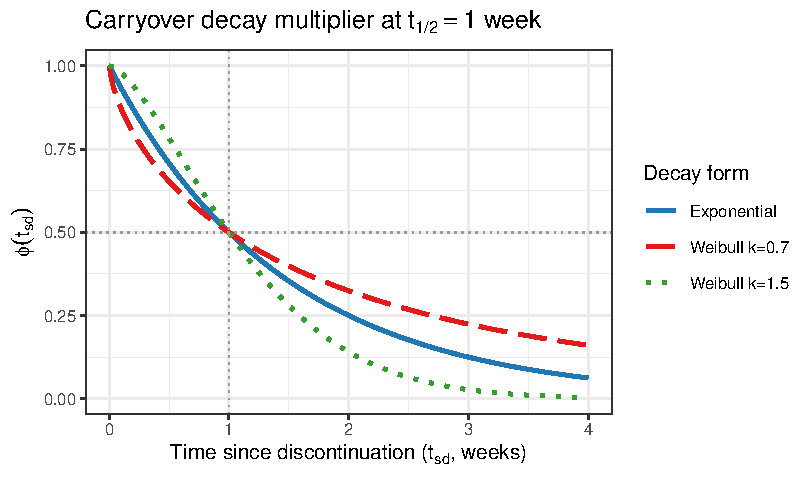
\includegraphics[width=0.7\linewidth]{../../figures/02xs-decay-curves} \caption{The carryover decay multiplier $\phi(t_{sd})$ at the reference half-life ($t_{1/2} = 1.0$ week) for exponential decay and the four Weibull shapes. The dotted reference lines mark the defining half-life point ($\phi = 0.5$ at $t_{sd} = t_{1/2}$), which all five curves pass through by construction; the shape parameter governs only how quickly $\phi$ falls before that point and how slowly it decays after.}\label{fig:fig-decay-curves}
\end{figure}

\begin{itemize}
\tightlist
\item
  Figure \ref{fig:fig-decay-curves} shows the shape difference
  concretely.
\item
  \(k = 0.25\) and \(k = 0.5\) curves have progressively heavier tails,
  staying well above the exponential curve for every \(t_{sd} >
  t_{1/2}\), most markedly at \(k = 0.25\).
\item
  Practical consequence: the analysis-side predictor picks up
  substantially more residual carryover during a prolonged washout
  than the half-life alone suggests, increasingly so as \(k\) falls
  further below one.
\item
  \(k = 2.0\) and \(k = 4.0\) curves have progressively lighter tails,
  clearing sharply faster once concentration falls below the
  half-maximum threshold.
\item
  All five curves pass through the same half-life-defining point
  (\(\phi = 0.5\) at \(t_{sd} = 1.0\)), so the five forms remain
  comparable at a fixed nominal half-life despite diverging shapes on
  either side of it.
\end{itemize}

\textbf{Section summary:}

\begin{itemize}
\tightlist
\item
  Two decay forms are used: exponential (the companion manuscript's
  form, first-order elimination kinetics) and Weibull, with a shape
  parameter \(k\) controlling tail weight relative to exponential.
\item
  Five decay-shape levels are examined in total (exponential plus
  four Weibull shapes, \(k \in \{0.25, 0.5, 2.0, 4.0\}\)); \(k=1.0\) is
  excluded as duplicating exponential.
\item
  All five decay curves are calibrated to the same half-life-defining
  point, so comparisons across shape are not confounded by a shifted
  half-life.
\end{itemize}

\subsection{Estimand and analysis specifications}\label{estimand-and-analysis-specifications}

\begin{itemize}
\tightlist
\item
  The interaction estimand is the on-drug biomarker-response
  correlation \(c_{bm}\), a dimensionless quantity.
\item
  Bias and empirical SE are reported on a calibrated effect-size
  scale (expected on-drug response difference per SD of biomarker at
  \(t_{1/2}=0\)), per \texttt{docs/19-mean-moderation-implementation-notes.tex}.
\item
  Power and Type I error are reported on the native test-statistic
  scale, with null estimand \(c_{bm} = 0\).
\item
  Shared model formula for the Tier 1 three: \texttt{nlme::lme(Sx\ \textasciitilde{}\ bm\ *\ X\ +\ t,\ random\ =\ \textasciitilde{}1\ \textbar{}\ ptID,\ correlation\ =\ corCAR1(form\ =\ \textasciitilde{}\ t\ \textbar{}\ ptID))},
  differing only in how \(X\) is constructed and whether a nuisance
  term is added.
\item
  Unadjusted and Lag-adjusted both test \(\text{bm:}D_{it}\), so every
  performance measure is comparable between them.
\item
  Exposure-weighted tests a different quantity, \(\text{bm:}D_{bc,it}\).

  \begin{itemize}
  \tightlist
  \item
    Power and Type I error remain comparable across all three
    specifications (properties of the test).
  \item
    Bias, MSE, and coverage are \textbf{not} comparable across that
    divide (cross-referenced to Section 3.1).
  \end{itemize}
\item
  Nine specifications total are evaluated across the manuscript:
  the Tier 1 three, plus six Tier 2 additions (introduced in the next
  section, tested in Blocks S7-S10, Section 3.7).
\item
  Internally (code and data files, Reproducibility section), each
  specification is stored under an \texttt{E}-prefixed code (\texttt{E1}, \texttt{E2},
  \ldots); the manuscript's prose refers to all nine uniformly by the
  compact \texttt{G1}-\texttt{G9} code (defined in \texttt{spec-labels.R}) or by name, per
  Table \ref{tab:tab-spec-summary} below.
\end{itemize}

\begin{table}
\centering
\caption{\label{tab:tab-spec-summary}All nine analysis specifications evaluated in this
    manuscript. G1-G3 are the Tier 1 headline three (Section 2.4);
    G4-G5 are Tier 2 additions replacing the retired E4/E5/E6
    (Blocks S7-S9, Section 3.7); G6-G9 are CR2 cluster-robust
    variants of G1, G2, G4, and G3 respectively (Block S10). G10
    (G5+CR2) does not apply and is omitted: G5 collapses to one row
    per patient before fitting, leaving no repeated-measures cluster
    structure for CR2 to correct.}
\centering
\resizebox{\ifdim\width>\linewidth\linewidth\else\width\fi}{!}{
\fontsize{9}{11}\selectfont
\begin{tabular}[t]{lllll}
\toprule
Code & Stored & Name & Formula & Target coefficient\\
\midrule
G1 & E1 & Unadjusted & Sx ~ bm + t + Db + bm:Db & bm:Db\\
G2 & E3 & Lag-adjusted & Sx ~ bm + t + Db + bm:Db + L & bm:Db\\
G3 & E2 & Exposure-weighted & Sx ~ bm + t + Dbc + bm:Dbc & bm:Dbc\\
G4 & E7 & AIC-selected t1/2 & G3 formula, t1/2 by AIC over \{0.25,0.5,1.0,2.0\} & bm:Dbc\\
G5 & E9 & Paired-difference & diff ~ bm (patient-level OLS) & bm slope\\
\addlinespace
G6 & E1cr2 & Unadjusted + CR2 & G1 formula, CR2 SE & bm:Db\\
G7 & E3cr2 & Lag-adjusted + CR2 & G2 formula, CR2 SE & bm:Db\\
G8 & E2cr2 & Exposure-weighted + CR2 & G3 formula, CR2 SE & bm:Dbc\\
G9 & E7cr2 & AIC-selected t1/2 + CR2 & G4 formula, CR2 SE & bm:Dbc\\
\bottomrule
\end{tabular}}
\end{table}

\subsubsection{Unadjusted (G1): binary on-drug indicator}\label{unadjusted-g1-binary-on-drug-indicator}

\begin{itemize}
\tightlist
\item
  \(X = D_{it}\), the binary on-drug indicator (one on drug, zero off).
\item
  Carryover is not represented at all.
\item
  An off-drug occasion still carrying most of the pharmacological
  effect is coded identically to one carrying none.
\item
  This is the default an analyst obtains without considering
  carryover; treated as the benchmark other specifications must
  justify their added structure against.
\item
  Consumes no half-life; invariant to the analyst's pharmacokinetic
  assumptions.
\end{itemize}

\subsubsection{Lag-adjusted (G2): binary indicator plus estimated carryover term}\label{lag-adjusted-g2-binary-indicator-plus-estimated-carryover-term}

\begin{itemize}
\tightlist
\item
  Retains \(X = D_{it}\); adds a lagged-treatment indicator,
  \(L_{it} = D_{i,t-1}(1 - D_{it})\), marking off-drug timepoints
  immediately following an on-drug one.
\item
  This is the classical crossover-trial device of Jones and Kenward\textsuperscript{\citeproc{ref-jones2014crossover}{4}}.
\item
  Carryover magnitude is estimated from the data, not assumed; like
  Unadjusted, this specification is invariant to the assumed
  half-life.
\item
  \(L_{it}\) enters only as a nuisance main effect; there is no
  \(\text{bm:}L_{it}\) product, so the interaction actually tested
  remains \(\text{bm:}D_{it}\).
\item
  Lag-adjusted can absorb mean-level carryover but cannot repair the
  interaction's attenuation (Section 1).
\item
  Framed as Unadjusted with a carryover nuisance control added, not a
  fundamentally different model of the interaction (Section 4.1).
\end{itemize}

\subsubsection{Exposure-weighted (G3): continuous decayed predictor}\label{exposure-weighted-g3-continuous-decayed-predictor}

\begin{itemize}
\tightlist
\item
  \(X = \text{Dbc}_{it}\), a continuous exposure-decayed predictor
  matched to the analyst's assumed decay form and half-life; the
  current pmsimstats-ng package default.
\item
  At on-drug timepoints, \(D_{bc,it} = 1\).
\item
  Off drug it decays as
  \(D_{bc,it} = (1/2)^{t_{sd,it}/\hat{t}_{1/2}}\), losing half its
  value every \(\hat{t}_{1/2}\) weeks after discontinuation.
\item
  When the assumed decay form matches the true one, the predictor is
  well matched; when it does not, it is mis-specified, probed
  directly in Block S2.
\item
  The half-life assumption enters only through the predictor values
  handed to \texttt{lme}, not the model formula, so this specification is in
  effect a different model for each assumed half-life.
\item
  It is the only one of the three original specifications that
  consumes a half-life at all; the S2 sensitivity contrast (Section
  3.7) is designed to probe this.
\item
  Limiting relationship: as \(\hat{t}_{1/2} \rightarrow 0\),
  \(D_{bc,it} \rightarrow D_{it}\), so Unadjusted is exactly the
  boundary member of the Exposure-weighted family at zero assumed
  half-life.
\item
  The S2 sweep is therefore a traverse anchored at Unadjusted, not an
  independent check.
\end{itemize}

\subsubsection{AIC-selected half-life (G4)}\label{aic-selected-half-life-g4}

\begin{itemize}
\tightlist
\item
  Uses Exposure-weighted's formula, \(X = \text{Dbc}_{it}\), but
  chooses \(\hat{t}_{1/2}\) from the data rather than assuming it.
\end{itemize}

\[
\hat{t}_{1/2} = \operatorname*{arg\,min}_{t_{1/2} \,\in\, \mathcal{T}}
  \text{AIC}\big(M(t_{1/2})\big), \qquad
  \mathcal{T} = \{0.25,\ 0.5,\ 1.0,\ 2.0\}\ \text{weeks},
\]

\begin{itemize}
\tightlist
\item
  \(\text{AIC}(M) = -2\log L(M) + 2p\), \(L(M)\) the fitted model's
  likelihood and \(p\) its number of estimated parameters\textsuperscript{\citeproc{ref-akaike1974new}{5}}.
\item
  Reported power, coefficient, and SE are read from
  \(M(\hat{t}_{1/2})\) alone, the single winning fit, not pooled or
  averaged across \(\mathcal{T}\).
\item
  Mirrors \texttt{characterize\_carryover()} (\texttt{R/carryover\_analysis.R}), the
  package's own real-data half-life-selection routine.
\item
  Like Exposure-weighted, targets \(\text{bm:}D_{bc,it}\); unlike
  Exposure-weighted, requires no half-life from the analyst at all.
\item
  Cost: a post-selection inference risk\textsuperscript{\citeproc{ref-berk2013valid}{6}} --
  \(M(\hat{t}_{1/2})\)'s reported SE and \(p\)-value treat
  \(\hat{t}_{1/2}\) as fixed in advance, when the same data in fact
  chose it, so nominal inference does not formally account for the
  selection step.
\item
  Block S11 (Section 3.7) checks whether this risk manifests as Type
  I error inflation in practice.
\end{itemize}

\subsubsection{Paired-difference (G5)}\label{paired-difference-g5}

\begin{itemize}
\tightlist
\item
  A two-stage, correlation-structure-agnostic alternative, not an
  elaboration of the mixed-model family above.
\item
  Stage 1: for each patient \(i\) with \(n_i^{\text{on}} > 0\) on-drug and
  \(n_i^{\text{off}} > 0\) off-drug occasions, define per-patient
  on-drug and off-drug means:
\end{itemize}

\[
\bar{S}_{x,i}^{\text{on}} = \frac{1}{n_i^{\text{on}}}
  \sum_{t:\, D_{it}=1} S_{x,it}, \qquad
\bar{S}_{x,i}^{\text{off}} = \frac{1}{n_i^{\text{off}}}
  \sum_{t:\, D_{it}=0} S_{x,it},
\]

\begin{itemize}
\tightlist
\item
  and their difference
  \(\Delta_i = \bar{S}_{x,i}^{\text{on}} - \bar{S}_{x,i}^{\text{off}}\).
\item
  Stage 2: OLS regression of \(\Delta_i\) on centered biomarker across
  \(N' \leq N\) patients contributing a difference:
\end{itemize}

\[
\Delta_i = \beta_0 + \beta_1\, bm_i + \varepsilon_i, \qquad
i = 1, \dots, N',
\]

\begin{itemize}
\tightlist
\item
  Interaction test is on \(\beta_1\).
\item
  No repeated-measures model, no carryover representation, no
  correlation structure of any kind: \(\Delta_i\) collapses each
  patient's eight occasions to one number before \(bm\) ever enters.
\item
  Framed as a direct biomarker-interaction extension of the paired
  t-test that Senn, Julious and Araujo\textsuperscript{\citeproc{ref-senn2014four}{7}} found to
  outperform carryover-adjusted mixed models for ordinary N-of-1
  treatment-effect estimation.
\item
  Patients contributing only on-drug or only off-drug observations
  (e.g., CO's never-discontinuing path) have \(n_i^{\text{on}} = 0\) or
  \(n_i^{\text{off}} = 0\), cannot form \(\Delta_i\), and are dropped, so
  \(N' < N\) whenever such a path exists in the design.
\end{itemize}

\subsubsection{CR2 cluster-robust variants (G6-G9)}\label{cr2-cluster-robust-variants-g6-g9}

\begin{itemize}
\tightlist
\item
  Section 3.6 (Block S6) shows the model-based interaction test is
  mildly conservative, and a CR2 bias-reduced cluster-robust SE
  restores nominal size without disturbing the ranking among G1-G3.
\item
  Uses the estimator of Bell and McCaffrey\textsuperscript{\citeproc{ref-bell2002bias}{8}}, via
  \texttt{clubSandwich}, paired with Satterthwaite degrees of freedom.
\item
  That correction (\texttt{lme+CR2} in Section 2.7) was applied only to G3
  there; Block S10 (Section 3.7) extends it to G1, G2, and G4 as
  well, replacing only the SE, reference distribution, and \(p\)-value
  on each specification's existing point estimate.
\item
  Mapping: G6 (G1+CR2), G7 (G2+CR2), G9 (G4+CR2).
\item
  G8 (G3+CR2) is the same specification already introduced in
  Section 2.7 and Block S6, carried into the nine-way comparison at
  Block S10 without rerunning it.
\item
  A tenth combination, G5+CR2, does not apply: G5 already collapses
  to one row per patient before fitting, leaving no repeated-measures
  cluster structure for CR2 to correct.
\end{itemize}

\textbf{Section summary:}

\begin{itemize}
\tightlist
\item
  Nine analysis specifications (G1-G9) are ultimately compared, built
  from three families: the Tier 1 three (Unadjusted, Lag-adjusted,
  Exposure-weighted), two Tier 2 additions (G4 AIC-selected half-life,
  G5 paired-difference), and CR2 cluster-robust variants (G6-G9) of
  the mixed-model specifications.
\item
  Unadjusted/Lag-adjusted share an estimand (\(\text{bm:}D_{it}\)) and
  so are directly comparable on every measure; Exposure-weighted,
  G4, G9 target a different estimand (\(\text{bm:}D_{bc,it}\)), so only
  power and Type I error are comparable across that divide.
\item
  G5 discards the mixed-model framework entirely in favor of a
  two-stage paired-difference regression, motivated by prior evidence
  that simplicity is not obviously costly in N-of-1 analysis.
\item
  Internally all nine specifications are stored under \texttt{E}-prefixed
  codes; the manuscript displays them uniformly as \texttt{G1}-\texttt{G9} via
  \texttt{spec-labels.R}.
\end{itemize}

\subsection{Choice of analysis specifications}\label{choice-of-analysis-specifications}

\begin{itemize}
\tightlist
\item
  Three considerations bounded which specifications were tested,
  rather than surveying the wider N-of-1/crossover-trial literature.
\item
  The Tier 1 three were chosen because each represents a distinct,
  established position an analyst can take toward unmeasured/assumed
  decay, not because they exhaust the space:

  \begin{itemize}
  \tightlist
  \item
    Unadjusted: the default any analyst obtains without considering
    carryover at all; necessary benchmark.
  \item
    Lag-adjusted: follows Jones and Kenward's\textsuperscript{\citeproc{ref-jones2014crossover}{4}} classical crossover-trial device.
  \item
    Exposure-weighted: the pmsimstats-ng package's own established
    default, so the practical stakes of getting its behavior right
    are correspondingly higher than for the other two.
  \end{itemize}
\item
  Untested alternative model classes, left out by design:

  \begin{itemize}
  \tightlist
  \item
    Bayesian hierarchical N-of-1 models.
  \item
    GEE and other marginal models (compared systematically, not just
    as a robustness check, per Section 2.7).
  \item
    Randomization and permutation tests.
  \item
    Functional or spline-based flexible decay curves.
  \item
    State-space or Kalman-filter treatments of drug concentration.
  \item
    Two-stage ``series of N-of-1 trials'' meta-analytic combination.
  \end{itemize}
\item
  This is a scoping decision, not an oversight: the manuscript's aim
  is to compare carryover \emph{representations} within a single, fixed
  conditional mixed-model framework matching Hendrickson's\textsuperscript{\citeproc{ref-hendrickson2020}{2}} original analysis model, not a comprehensive
  methods bake-off (future work: Section 4.6).
\item
  Blocks S7-S9 (Section 3.7) revisit this scoping decision once, for
  a specific reason: Section 4.1 shows no carryover term tested so
  far can repair the interaction's attenuation as long as it enters
  only as a nuisance main effect; the natural next model interacts
  the carryover term with the biomarker directly.
\item
  An earlier version of Block S7 tested two such interacted
  specifications:

  \begin{itemize}
  \tightlist
  \item
    \texttt{E5}: a lagged term crossed with \texttt{bm}.
  \item
    \texttt{E6}: a continuous elapsed-time term crossed with \texttt{bm}.
  \end{itemize}
\item
  Both underperformed Unadjusted at every cell examined, across three
  blocks, two trial designs, two architectures, and three carryover
  half-lives (Sections 3.6, 4.5).
\item
  Traced to a structural cause: the DGP has a single true decay
  parameter, so crossing a second carryover term with the biomarker
  adds a free parameter with no counterpart in the truth being
  estimated; two collinear regressors chasing one true degree of
  freedom lose power to a correctly specified single-parameter model
  almost by construction.
\item
  A further variant of the same interacted-term family is expected to
  fail on the same structural argument, so \texttt{E5}/\texttt{E6} were replaced by
  two specifications answering different open questions about the
  analyst's unknown true decay half-life:

  \begin{itemize}
  \tightlist
  \item
    \texttt{G4} asks whether estimating the half-life from the data recovers
    the power a correctly assumed half-life would give; selects by
    AIC over a candidate grid, reusing the logic of
    \texttt{characterize\_carryover()} (\texttt{R/carryover\_analysis.R}), already
    used for real-data analysis; addresses Block S2's question from
    the opposite direction (estimation instead of assumption).
  \item
    \texttt{G5} asks a more basic question raised by the wider literature:
    is a conditional mixed model even necessary? Senn, Julious and
    Araujo\textsuperscript{\citeproc{ref-senn2014four}{7}} compared four analysis strategies for
    ordinary N-of-1 trials and found a simple paired t-test on
    within-patient treatment differences achieved near-nominal Type I
    error, higher power, and comparable bias/MSE relative to a
    carryover-adjusted mixed model, recommending the mixed model only
    when carryover is specifically suspected. \texttt{G5} is a direct
    biomarker-interaction extension of their preferred method.
  \end{itemize}
\item
  This remains a bounded comparison: \texttt{G4} and \texttt{G5} were chosen because
  each is implementable within, or trivially adjacent to, the
  existing analysis pipeline (Section 2.7), and each answers a
  specific question the manuscript's own results raised, not because
  they close the wider literature gap.
\item
  Bayesian, GEE-as-primary-model, randomization-test, and two-stage
  meta-analytic alternatives remain untested and are discussed as
  future work (Section 4.6).
\end{itemize}

\textbf{Section summary:}

\begin{itemize}
\tightlist
\item
  The Tier 1 three specifications were chosen as distinct, established
  analyst positions, not as an exhaustive survey of the N-of-1
  literature; a wide range of model classes was left untested by
  deliberate scoping decision.
\item
  An earlier interacted-carryover-term family (\texttt{E5}/\texttt{E6}) failed
  structurally because the DGP has a single true decay parameter, and
  was replaced by \texttt{G4} (AIC-selected half-life) and \texttt{G5}
  (paired-difference regression), each targeting the analyst's
  unknown-half-life problem from a different angle.
\item
  \texttt{G4} and \texttt{G5} remain a bounded addition, not a comprehensive methods
  comparison; several major alternative frameworks (Bayesian, GEE,
  randomization tests, two-stage meta-analysis) are explicitly
  deferred to future work.
\end{itemize}

\subsection{Factorial grid and parameter settings}\label{factorial-grid-and-parameter-settings}

\begin{itemize}
\tightlist
\item
  The principal comparison crosses biomarker moderation, carryover
  half-life, trial design, and sample size against the three Tier-1
  analysis specifications, under covariance moderation and the
  exponential DGP.
\end{itemize}

{\def\LTcaptype{none} % do not increment counter
\begin{longtable}[]{@{}ll@{}}
\toprule\noalign{}
Parameter & Values \\
\midrule\noalign{}
\endhead
\bottomrule\noalign{}
\endlastfoot
Biomarker moderation (\(c_{bm}\)) & 0.0, 0.30, 0.45 \\
Carryover half-life (\(t_{1/2}\)) & 0.0, 0.5, 1.0 weeks \\
Sample size (\(N\)) & 35, 70 \\
Trial design & CO, N-of-1 (Hybrid), OL+BDC \\
DGP architecture & B (covariance moderation) only \\
Replicates per cell & 500 (target), 50 for development \\
\end{longtable}
}

\begin{itemize}
\tightlist
\item
  Three specifications, three half-lives, three designs, two sample
  sizes, three biomarker levels: \(3 \times 3 \times 3 \times 2 \times
  3 = 162\) cells.
\item
  The \(c_{bm} = 0\) row is the Type I error check against nominal 5\%.
\item
  The \(t_{1/2} = 0\) row (no carryover) gives a best-case power
  reference at each combination of \(N\), design, and \(c_{bm}\), against
  which the cost of nonzero carryover can be read off directly.
\item
  Decay-shape sensitivity (Figures 3 and 5) is evaluated separately,
  at the reference cell only (\(c_{bm} = 0.45\), \(t_{1/2} = 1.0\)
  weeks), not across the full grid:

  \begin{itemize}
  \tightlist
  \item
    Exponential decay and four Weibull shapes (\(k \in \{0.25, 0.5,
    2.0, 4.0\}\), Section 2.3) crossed with three specifications,
    three designs, two sample sizes give \(5 \times 3 \times 3 \times
    2 = 90\) further cells (\texttt{23-run-decay-shape-sensitivity.R}).
  \end{itemize}
\item
  Rationale for restricting the decay-shape axis to one cell: it is
  the axis every other result in this manuscript holds fixed at
  exponential, and a full crossing would multiply simulation cost
  several times over for a comparison used in only two figures.
\item
  \(k = 1.0\) is not a fifth Weibull condition anywhere in this
  manuscript: it recovers the exponential form exactly (Section 2.3).
\end{itemize}

\textbf{Section summary:}

\begin{itemize}
\tightlist
\item
  The principal factorial grid has 162 cells crossing \(c_{bm}\),
  \(t_{1/2}\), \(N\), and trial design against the three Tier-1
  specifications, plus a separate 90-cell decay-shape sensitivity
  grid evaluated only at the reference cell.
\item
  The \(c_{bm}=0\) row anchors Type I error checks; the \(t_{1/2}=0\) row
  anchors the best-case (no-carryover) power reference used
  throughout the Results.
\end{itemize}

\subsection{Inference and the cluster-robust correction}\label{sec-cr2}

\begin{itemize}
\tightlist
\item
  The interaction test described so far is model-based: the SE of
  \(\beta_{bm:X}\) is read from the fitted \texttt{lme} object, valid only if
  the assumed residual covariance is correct.
\item
  This assumption is not innocuous: the working covariance (patient
  random intercept plus \texttt{corCAR1} AR(1) residual correlation) does
  not match the covariance the DGP actually induces\textsuperscript{\citeproc{ref-pmsimstats_calibration2026}{9}}, inflating the SE by roughly six to
  ten percent and depressing the rejection rate correspondingly.
\end{itemize}

\[
\kappa = \frac{\overline{\widehat{SE}}}{SD\big(\hat\beta_{bm:X}\big)}
       = \frac{\frac{1}{n_{sim}}\sum_{r=1}^{n_{sim}} \widehat{SE}_r}
              {\sqrt{\frac{1}{n_{sim}-1}\sum_{r=1}^{n_{sim}}
                \big(\hat\beta_{bm:X,r} - \bar{\hat\beta}_{bm:X}\big)^2}},
\]

\begin{itemize}
\tightlist
\item
  \(\kappa\) is the mean model-reported SE across replicates divided by
  the empirical SD of replicate-level point estimates.

  \begin{itemize}
  \tightlist
  \item
    \(\kappa = 1\): correctly calibrated.
  \item
    \(\kappa > 1\): model overstates uncertainty (a conservative test).
  \end{itemize}
\item
  At the null cell, \(\kappa\) runs 1.05 to 1.10 across specifications,
  with empirical Type I error 0.029 to 0.039 against nominal 0.05.
\item
  Remedy: a cluster-robust (sandwich) variance estimator, valid under
  covariance mis-specification, deriving variance from observed
  between-cluster variation rather than the assumed covariance.
\item
  Clusters are patients (eight occasions each, unique across
  randomization paths).
\end{itemize}

\[
\widehat{\text{Var}}_{\text{sandwich}}(\hat\beta) =
  \left(\sum_{i=1}^{N} X_i' \hat{V}_i^{-1} X_i\right)^{-1}
  \left(\sum_{i=1}^{N} X_i' \hat{V}_i^{-1} \hat{e}_i \hat{e}_i'
    \hat{V}_i^{-1} X_i\right)
  \left(\sum_{i=1}^{N} X_i' \hat{V}_i^{-1} X_i\right)^{-1},
\]

\begin{itemize}
\tightlist
\item
  This naive (Liang-Zeger) sandwich estimator substitutes each
  patient's own observed \(\hat{e}_i\hat{e}_i'\) for the single assumed
  \(\hat{V}_i\), so a mismatched working covariance no longer biases the
  variance estimate -- at the cost of needing enough clusters for
  stability.
\item
  With only \(N = 35\) or \(70\) clusters, the naive sandwich form is
  itself markedly downward-biased, so the CR2 bias-reduced estimator
  of Bell and McCaffrey\textsuperscript{\citeproc{ref-bell2002bias}{8}} is used instead.
\item
  CR2 replaces each raw residual \(\hat{e}_i\) with an adjusted residual
  \(\hat{e}_i^{\text{CR2}} = A_i \hat{e}_i\), chosen so the recomputed
  sandwich variance is exactly unbiased under the working model (full
  construction of \(A_i\) in Bell and McCaffrey\textsuperscript{\citeproc{ref-bell2002bias}{8}}, not
  reproduced here).
\item
  Paired with Satterthwaite degrees of freedom (both via
  \texttt{clubSandwich}); replaces only SE, reference distribution, and
  \(p\)-value, leaving point estimates untouched.
\item
  The correction is applied in two places:

  \begin{itemize}
  \tightlist
  \item
    A null-cell diagnostic (\(c_{bm} = 0\), exponential DGP,
    \(t_{1/2} = 1.0\) weeks, Hybrid, \(N = 70\), 3,000 replicates)
    establishing whether CR2 restores nominal size (Section 3.6).
  \item
    A five-cell block (reference cell plus four stress cells: small
    \(N\), high autocorrelation, half-life mis-specification, 30\% MCAR
    dropout; 500 replicates each; labeled S6), asking whether
    restoring size disturbs the ranking (same section).
  \end{itemize}
\item
  Blocks S1-S4 are the Tier 2 sensitivity analyses of Section 3.7.
\item
  Block S5 (exploratory autocorrelation-by-carryover interaction) is
  outside the present scope, reported only in the archived
  full-scope drafts.
\end{itemize}

\textbf{Section summary:}

\begin{itemize}
\tightlist
\item
  The default model-based interaction test is mildly conservative
  because the working covariance does not match the true
  data-generating covariance, quantified by the calibration ratio
  \(\kappa\) (1.05-1.10 at the null cell).
\item
  A CR2 bias-reduced cluster-robust SE (Bell and McCaffrey), paired
  with Satterthwaite degrees of freedom, is the chosen remedy,
  applied at a null-cell diagnostic and a five-cell stress block
  (S6).
\item
  Blocks S1-S5 constitute the remaining Tier 2 sensitivity analyses;
  S5 is out of scope here and reported only in archived drafts.
\end{itemize}

\subsection{Performance measures and computing environment}\label{performance-measures-and-computing-environment}

\begin{itemize}
\tightlist
\item
  Reported per cell: Power, Type I error, Bias, Empirical SE
  (calibrated scale), Coverage of the nominal 95\% Wald CI, MSE,
  non-convergence rate, and the MCSE of each, following Morris et al.\textsuperscript{\citeproc{ref-morris2019simulation}{1}, Tables 5-6}.
\item
  \(n_{sim} = 500\) chosen so the MCSE on power at \(p = 0.5\) would not
  exceed 0.022.
\item
  No simulation runs for this manuscript at render time; it filters
  the same 540-cell production grid summary used in the archived
  full-scope drafts down to the 216-cell slice defined by covariance
  moderation and the two non-linear decay forms.
\item
  All three specifications are fit to the same simulated dataset
  within each cell (common random numbers), so every pairwise
  contrast -- especially Lag-adjusted minus Unadjusted -- carries
  reduced Monte Carlo variance relative to independent draws.
\item
  The Tier 2 sensitivity blocks and S6 recalibration are filtered
  from the same shared production outputs.
\item
  Exact file paths and versions are given in the Reproducibility
  section.
\end{itemize}

\textbf{Section summary:}

\begin{itemize}
\tightlist
\item
  Performance is reported on the standard Morris et al.~ADEMP measure
  set, with \(n_{sim}=500\) calibrated to an MCSE ceiling of 0.022 on
  power.
\item
  This manuscript performs no new simulation at render time; it reads
  and filters existing production outputs, relying on common random
  numbers across specifications to sharpen pairwise contrasts.
\end{itemize}

\section{Results}\label{results}

\begin{itemize}
\tightlist
\item
  All reported results derive from the same 500-replicate production
  run used in the full-scope manuscripts, filtered to the
  covariance-moderation architecture and the exponential and Weibull
  decay forms.
\item
  The Monte Carlo SE on power does not exceed 0.022 at \(p = 0.5\);
  differences smaller than this should not be over-interpreted.
\item
  Coverage of the nominal 95\% Wald CI is reported for the reference
  cell.
\item
  Non-convergence rates are reported per cell in the tables that
  follow.
\end{itemize}

\textbf{Section summary:}

\begin{itemize}
\tightlist
\item
  Every Results figure and table is drawn from a single 500-replicate
  production run (covariance moderation, exponential/Weibull decay
  only), with an MCSE ceiling of 0.022 on power that should be used
  to judge whether any reported gap is meaningful.
\end{itemize}

\subsection{Headline performance table}\label{sec-headline}

\begin{itemize}
\tightlist
\item
  Table \ref{tab:headline} reports performance at the reference cell
  (exponential DGP, Hybrid design, \(N = 70\), \(c_{bm} = 0.45\)), where
  non-convergence was zero throughout.
\item
  Bias, MSE, and coverage columns are computed against
  Exposure-weighted's calibrated target,
  \(\theta_{\text{true}} = -c_{bm}\sigma_{BR} = -3.6\).
\item
  Unadjusted and Lag-adjusted estimate a different coefficient,
  \(\text{bm:}D_{it}\); their apparent bias and under-coverage reflect
  this estimand mismatch, not an estimator defect.
\item
  Those columns are comparable within the Unadjusted/Lag-adjusted
  pair but not across to Exposure-weighted.
\item
  For the three-way comparison, power and Type I error (properties of
  the test rather than the coefficient) are the measures to rely on.
\end{itemize}

\begin{table}
\centering
\caption{\label{tab:headline}Headline performance at the reference cell
    (exponential DGP, Hybrid design, $N = 70$,
    $c_{bm} = 0.45$, $n_{sim} = 500$). Power is the rejection rate of
    $H_0: \beta_{bm:X} = 0$ at $\alpha = 0.05$, the primary outcome
    of this manuscript. Bias is mean(estimate $-$
    $\theta_{\text{true}}$) on the calibrated effect-size scale,
    $\theta_{\text{true}} = -c_{bm} \cdot \sigma_{BR} = -3.6$
    (per docs/19 calibration; see the estimand-mismatch caveat above
    for Unadjusted/Lag-adjusted). Empirical SE is the standard
    deviation of the point estimates across replicates, the actual
    sampling variability of the estimator, as distinct from
    whatever SE any single fit reports (the comparison the
    calibration ratio $\kappa$ of Section 2.7 is built on). Coverage
    is the proportion of replicates whose nominal 95\% Wald CI
    contains $\theta_{\text{true}}$; the low Unadjusted/Lag-adjusted
    values reflect the same estimand mismatch as Bias, not
    miscalibrated inference. MSE is bias$^2$ + Empirical SE$^2$, an
    overall accuracy summary. Non-conv is the fraction of replicates
    where `nlme::lme()` failed to converge (zero throughout at this
    cell). MCSEs are reported per Morris et al. (2019, Table 6).}
\centering
\resizebox{\ifdim\width>\linewidth\linewidth\else\width\fi}{!}{
\begin{tabular}[t]{rlllllll}
\toprule
t1/2 & Specification & Power (MCSE) & Bias (MCSE) & Empirical SE & Coverage (MCSE) & MSE (MCSE) & Non-conv\\
\midrule
0.0 & Unadjusted & 0.988 (0.005) & -0.029 (0.033) & 0.746 & 0.990 (0.004) & 0.557 (0.034) & 0.000\\
0.0 & Lag-adjusted & 0.990 (0.004) & -0.025 (0.033) & 0.746 & 0.990 (0.004) & 0.557 (0.034) & 0.000\\
0.0 & Exposure-weighted & 0.988 (0.005) & -0.029 (0.033) & 0.746 & 0.990 (0.004) & 0.557 (0.034) & 0.000\\
0.5 & Unadjusted & 0.918 (0.012) & +0.586 (0.036) & 0.807 & 0.938 (0.011) & 0.995 (0.058) & 0.000\\
0.5 & Lag-adjusted & 0.920 (0.012) & +0.583 (0.036) & 0.812 & 0.938 (0.011) & 1.000 (0.059) & 0.000\\
\addlinespace
0.5 & Exposure-weighted & 0.948 (0.010) & +0.072 (0.041) & 0.907 & 0.972 (0.007) & 0.828 (0.057) & 0.000\\
1.0 & Unadjusted & 0.766 (0.019) & +1.093 (0.038) & 0.847 & 0.828 (0.017) & 1.911 (0.093) & 0.000\\
1.0 & Lag-adjusted & 0.770 (0.019) & +1.099 (0.038) & 0.853 & 0.818 (0.017) & 1.935 (0.094) & 0.000\\
1.0 & Exposure-weighted & 0.860 (0.016) & -0.081 (0.049) & 1.085 & 0.968 (0.008) & 1.184 (0.077) & 0.000\\
\bottomrule
\end{tabular}}
\end{table}

\textbf{Section summary:}

\begin{itemize}
\tightlist
\item
  The headline table anchors the manuscript's reference cell
  (exponential, Hybrid, \(N=70\), \(c_{bm}=0.45\)); bias/MSE/coverage
  columns are valid only within the Unadjusted/Lag-adjusted pair or
  within Exposure-weighted alone, because the two families target
  different estimands.
\item
  Power and Type I error are the only measures directly comparable
  across all three Tier-1 specifications.
\end{itemize}

\subsection{Tier 1 grid overview}\label{tier-1-grid-overview}

\begin{itemize}
\tightlist
\item
  Figures \ref{fig:fig-hendrickson-a} through
  \ref{fig:fig-hendrickson-c} give a full-grid heatmap view of the
  Tier 1 results: trial design as column facets, \(N\) as row-block
  facets, analysis specification as the row axis within each block,
  blue-to-red fill scale for power.
\item
  Each panel fixes two grid dimensions and varies a third, since no
  single 2D heatmap can display all four simultaneously.
\item
  Panels A and B report all nine G1-G9 specifications (a dedicated
  simulation restricted to exponential DGP and Architecture B,
  \(n_{sim} = 100\), preliminary).
\item
  Panel C retains the original three (G1-G3), the only panel varying
  DGP decay form, an axis the G1-G9 extension did not re-run.
\end{itemize}

\begin{figure}
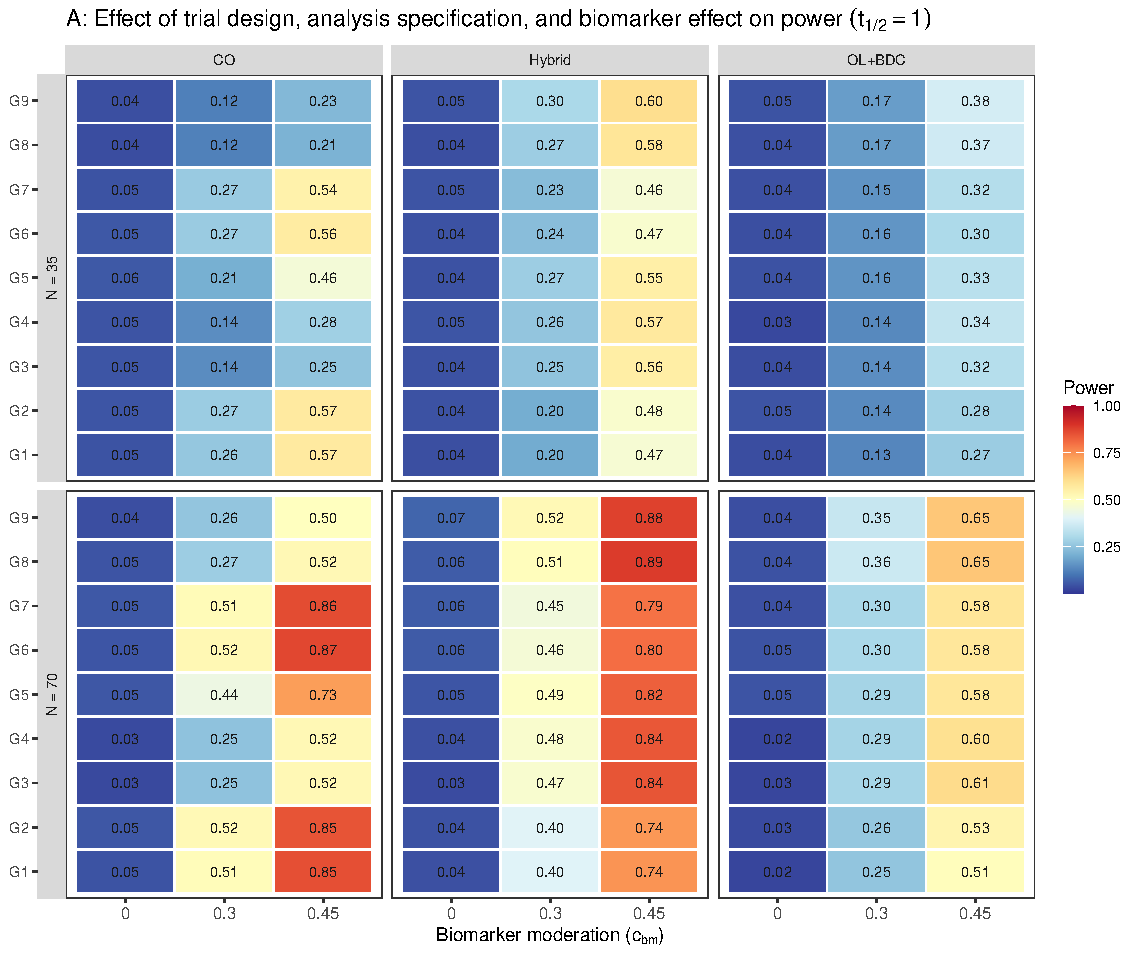
\includegraphics[width=0.95\linewidth]{../../figures/02xs-heatmap-hendrickson-a} \caption{Tier 1 grid, biomarker-effect axis, all nine G1-G9 specifications: power by trial design (columns), $N$ (row blocks), and analysis specification (rows within block), across $c_{bm} \in \{0, 0.30, 0.45\}$ at $t_{1/2} = 1.0$ weeks, exponential DGP, Architecture B (preliminary $n_{sim} = 100$).}\label{fig:fig-hendrickson-a}
\end{figure}

\begin{itemize}
\tightlist
\item
  Two features visible at a glance in Panel A that the headline table
  only shows cell by cell:

  \begin{itemize}
  \tightlist
  \item
    \texttt{G1} and \texttt{G2} track each other closely at every biomarker level
    within every design/\(N\) block, differing by at most 0.03 (within
    Monte Carlo noise at this preliminary \(n_{sim}=100\)), matching
    the higher-precision Section 3.4 result of numerical identity to
    two decimal places.
  \item
    The Exposure-weighted family (\texttt{G3}, \texttt{G4}, and CR2 variants \texttt{G8},
    \texttt{G9}) separates from \texttt{G1}/\texttt{G2}/\texttt{G6}/\texttt{G7} only in Hybrid and OL+BDC
    columns; in the CO column the whole family underperforms at every
    biomarker level past zero.
  \end{itemize}
\item
  At the reference cell (\(c_{bm}=0.45\), \(t_{1/2}=1.0\)): \texttt{G4} reaches
  0.48 against 0.86-0.89 for \texttt{G1}/\texttt{G2}/\texttt{G6}/\texttt{G7} -- the
  design-dependence of Section 3.4, now visible across all nine
  specifications.
\item
  Whether this separation depends on carryover being present at all
  cannot be shown by Panel A alone, since it fixes \(t_{1/2}=1.0\)
  throughout.
\end{itemize}

\begin{figure}
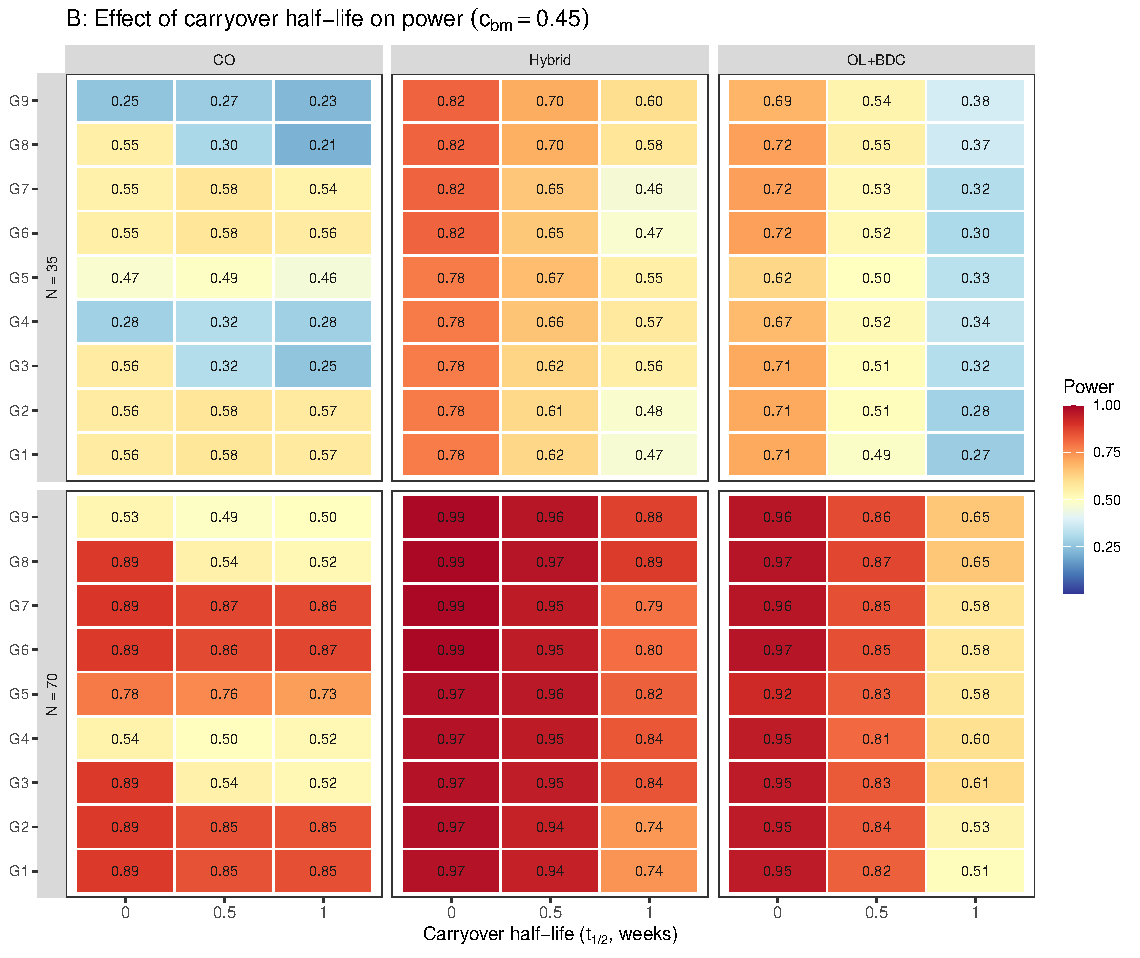
\includegraphics[width=0.95\linewidth]{../../figures/02xs-heatmap-hendrickson-b} \caption{Tier 1 grid, carryover-axis, all nine G1-G9 specifications: power by trial design (columns), $N$ (row blocks), and analysis specification (rows within block), across $t_{1/2} \in \{0, 0.5, 1.0\}$ weeks at $c_{bm} = 0.45$, exponential DGP, Architecture B (preliminary $n_{sim} = 100$).}\label{fig:fig-hendrickson-b}
\end{figure}

\begin{itemize}
\tightlist
\item
  Panel B answers the above, for Hybrid and OL+BDC:

  \begin{itemize}
  \tightlist
  \item
    At \(t_{1/2}=0\) the Exposure-weighted family's separation from
    \texttt{G1}/\texttt{G2}/\texttt{G6}/\texttt{G7} disappears in both designs (all nine sit at
    0.94-1.00), opening up only as half-life increases -- confirming
    the separation is specifically a carryover effect.
  \item
    Under CO the picture differs: \texttt{G4} and \texttt{G9} are already collapsed
    at \(t_{1/2}=0\) (0.48 and 0.47, against 0.88-0.92 for the rest),
    before carryover enters at all -- the AIC mis-selection pathology
    of Block S9, predating \(t_{1/2}>0\) rather than growing from it.
  \end{itemize}
\item
  Ranking result from Panel B: \texttt{G9} and \texttt{G8} lead in a near-tie at
  Hybrid and OL+BDC reference cells (both around 0.88 at Hybrid, 0.77
  to 0.74 at OL+BDC).
\item
  \texttt{G5} (Paired-difference) is the strongest non-\texttt{G1}/\texttt{G2}/CR2-variant
  specification at CO (0.77, versus 0.48-0.51 for the
  Exposure-weighted family there), consistent with \texttt{G5} discarding
  the carryover representation that costs the Exposure-weighted
  family power under CO.
\end{itemize}

\begin{figure}
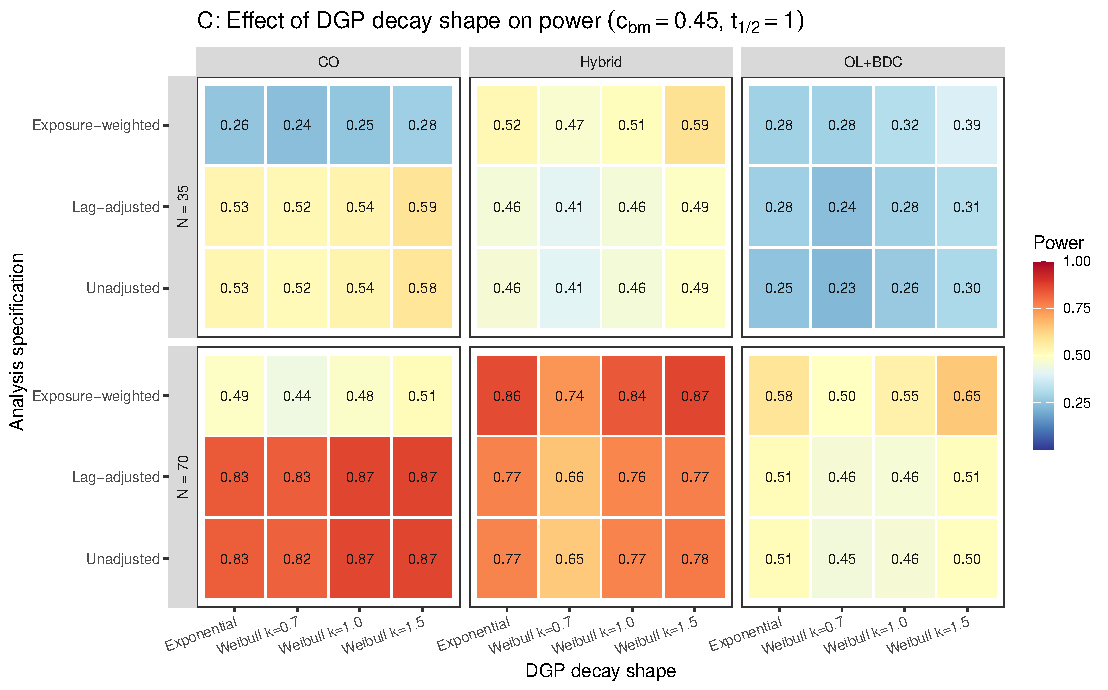
\includegraphics[width=0.95\linewidth]{../../figures/02xs-heatmap-hendrickson-c} \caption{Tier 1 grid, decay-shape axis: power by trial design (columns), $N$ (row blocks), and analysis specification (rows within block), across the five DGP decay-shape levels (exponential, Weibull $k \in \{0.25, 0.5, 2.0, 4.0\}$) at $c_{bm} = 0.45$, $t_{1/2} = 1.0$ weeks.}\label{fig:fig-hendrickson-c}
\end{figure}

\begin{itemize}
\tightlist
\item
  Panel C shows the Exposure-weighted row's advantage in Hybrid and
  OL+BDC columns is not uniform across decay shape:

  \begin{itemize}
  \tightlist
  \item
    Widens substantially on the light-tailed side (\(k=2.0\), \(4.0\)),
    reaching \(+0.14\) to \(+0.21\) absolute over Unadjusted/Lag-adjusted
    at OL+BDC.
  \item
    Narrows on the heavy-tailed side, disappearing at the two most
    extreme shapes (\(k=0.25\), \(0.5\)): statistically indistinguishable
    at OL+BDC (gaps of \(0.00\) to \(0.02\), well under one MCSE), barely
    separated at Hybrid (\(+0.01\) to \(+0.04\)).
  \end{itemize}
\item
  This is the decay-form sensitivity of Section 3.5, shown here
  across the full grid rather than at one cell.
\end{itemize}

\textbf{Section summary:}

\begin{itemize}
\tightlist
\item
  The three-panel Tier 1 heatmap view confirms, across the full grid,
  that G1/G2 are numerically indistinguishable everywhere, and that
  the Exposure-weighted family's advantage is confined to Hybrid/
  OL+BDC designs, growing with carryover severity, and dependent on
  decay-shape assumptions.
\item
  CO is uniformly unfavorable to the Exposure-weighted family, with
  \texttt{G4}/\texttt{G9} showing an AIC mis-selection pathology visible even
  without carryover (\(t_{1/2}=0\)).
\end{itemize}

\subsection{Matched-decay baseline}\label{matched-decay-baseline}

\begin{itemize}
\tightlist
\item
  At the matched cell (exponential DGP, exposure-weighted analysis,
  \(N=70\), \(c_{bm}=0.45\), Hybrid design), power declines:

  \begin{itemize}
  \tightlist
  \item
    \(0.988 \pm 0.005\) at \(t_{1/2}=0\).
  \item
    \(0.948 \pm 0.010\) at \(t_{1/2}=0.5\).
  \item
    \(0.860 \pm 0.016\) at \(t_{1/2}=1.0\) weeks.
  \item
    (point estimate \(\pm\) MCSE, \(n_{sim}=500\); all 500 replicates
    converged at every half-life in this cell)
  \end{itemize}
\item
  A previously reported comparison to Hendrickson et al.'s power of
  0.82 for a comparable cell\textsuperscript{\citeproc{ref-hendrickson2020}{2}} is withdrawn.
\item
  Reason: in the reference implementation, analysis-side and
  data-generating carryover parameters are set independently; the
  drivers reproducing the original figures supply a half-life only to
  the data-generating step, leaving the analysis-side half-life at
  its default of zero.
\item
  At a zero half-life, the exposure-decayed predictor collapses onto
  the binary on-drug indicator, so the reference analysis is actually
  Unadjusted, not Exposure-weighted.
\item
  The appropriate comparator is therefore the unadjusted power at the
  same cell, \(0.766\).
\item
  The grids also differ further on interaction strength and
  half-life, so ``the same cell'' was approximate in any case.
\item
  What the published figure was computed under has not been
  resolved; no claim of agreement or disagreement is made.
\item
  This does not affect the rest of the manuscript, since analysis
  specifications are compared against one another within a single
  simulation under common random numbers.
\end{itemize}

\textbf{Section summary:}

\begin{itemize}
\tightlist
\item
  A previously claimed numerical match to Hendrickson et al.'s
  published power (0.82) is withdrawn: the reference implementation's
  half-life default of zero means the true comparator is the
  Unadjusted power (0.766), not Exposure-weighted.
\item
  This unresolved external-comparison issue does not affect any
  internal comparison in the manuscript.
\end{itemize}

\subsection{Power by analysis specification}\label{power-by-analysis-specification}

\begin{figure}
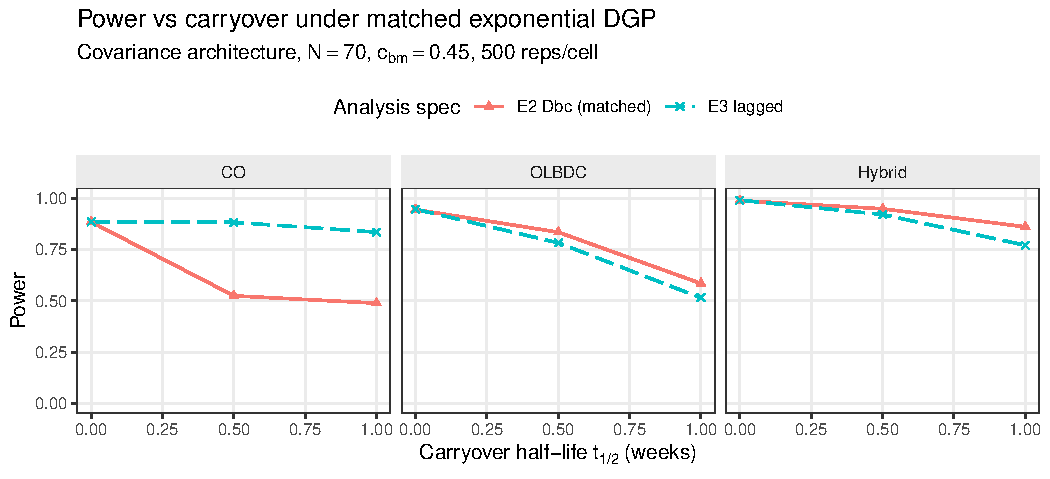
\includegraphics[width=0.95\linewidth]{../../figures/02xs-power-by-spec} \caption{Power versus carryover half-life under the exponential DGP, by analysis specification and trial design.}\label{fig:fig-power-by-spec}
\end{figure}

\begin{itemize}
\tightlist
\item
  Two features of Figure \ref{fig:fig-power-by-spec} carry the
  substance of this study:

  \begin{itemize}
  \tightlist
  \item
    Unadjusted and Lag-adjusted curves lie on top of one another in
    every panel and every half-life: \(0.766\) and \(0.770\) at
    \(t_{1/2}=1.0\) weeks at the reference cell; across all 216 cells
    the mean difference is 0.003, with mean bias, MSE, coverage
    agreeing to three decimal places. This is read as a clean null:
    the two share an estimand, are fitted to the same simulated
    datasets, and differ by exactly one nuisance term (the
    lagged-treatment term contributes nothing, Section 4.1).
  \item
    The three specifications give nearly identical power at
    \(t_{1/2}=0\) (no carryover), diverging as half-life increases, with
    Exposure-weighted separating from the other two.
  \end{itemize}
\item
  Exposure-weighted retains a modest but consistent advantage in
  Hybrid and OL+BDC designs from \(t_{1/2}=0.5\) weeks onward.
\item
  Under crossover, Exposure-weighted is markedly inferior to both
  alternatives (\(0.488\) against \(0.830\) for Unadjusted).
\item
  Proposed mechanism: the within-subject correlation in a crossover
  trial already carries most of the signal the decaying predictor
  targets, so it gains little there while its down-weighting of
  off-drug observations works against it (Section 4).
\end{itemize}

\textbf{Section summary:}

\begin{itemize}
\tightlist
\item
  Unadjusted and Lag-adjusted are statistically indistinguishable at
  every half-life and every design, the manuscript's cleanest null
  result.
\item
  Exposure-weighted's advantage over the other two grows with
  half-life in Hybrid/OL+BDC but reverses sharply under crossover
  (0.488 vs 0.830), attributed to crossover's within-subject
  correlation already capturing the signal the decayed predictor
  targets.
\end{itemize}

\subsection{Decay-form mis-specification}\label{decay-form-mis-specification}

\begin{figure}
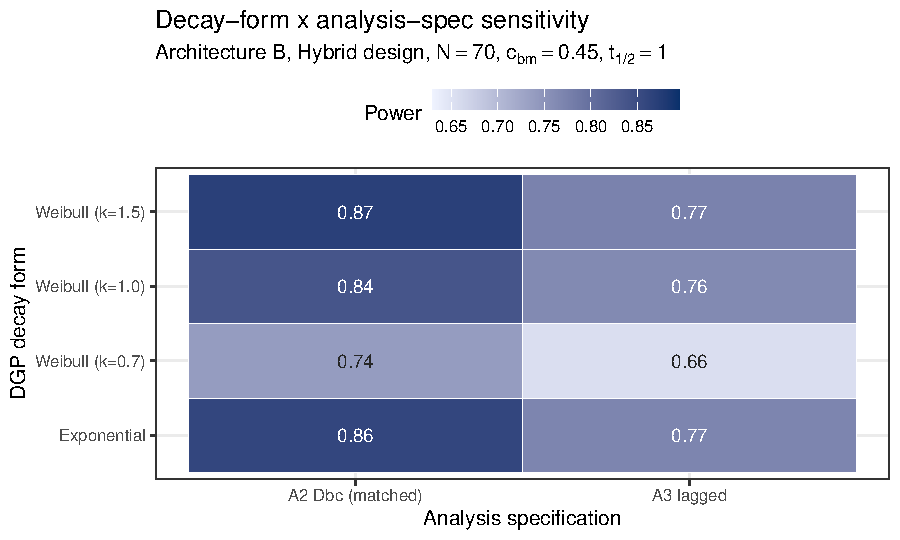
\includegraphics[width=0.85\linewidth]{../../figures/02xs-heatmap-matched-vs-mismatched} \caption{Power at the critical cell ($t_{1/2} = 1.0$ weeks, Hybrid, $N = 70$, $c_{bm} = 0.45$) across five DGP decay forms (rows) and specifications (columns). Fill scale is stretched to the observed range, not [0,1], and not comparable to other figures.}\label{fig:fig-heatmap-mismatch}
\end{figure}

\begin{itemize}
\tightlist
\item
  The exponential-DGP/Exposure-weighted cell is the matched reference,
  power \(0.850 \pm 0.016\) in this figure's own (dedicated
  decay-shape) simulation; the \(0.860\) reported for the nominally
  same cell in Table \ref{tab:headline} and Figure
  \ref{fig:fig-power-by-spec} comes from an independent draw of the
  same DGP, agreeing within one MCSE.
\item
  Unadjusted and Lag-adjusted columns, invariant to assumed decay form
  by construction, are near-identical throughout, so variation down
  those columns reflects data-generating decay and Monte Carlo noise
  only.
\item
  The Exposure-weighted row gives the cost of assuming exponential
  decay when the truth is Weibull, and it is asymmetric:

  \begin{itemize}
  \tightlist
  \item
    Light-tailed side (\(k=2.0\)): \(0.880\) against \(0.788\) for both
    alternatives (\(+0.092\)).
  \item
    Light-tailed side (\(k=4.0\)): \(0.930\) against \(0.786\)/\(0.788\)
    (\(+0.142\) to \(+0.144\)).
  \item
    Heavy-tailed side (\(k=0.5\)): \(0.708\) against \(0.676\) and
    \(0.672\) (\(+0.032\) to \(+0.036\), roughly 1.5 MCSE).
  \item
    Heavy-tailed side (\(k=0.25\), most extreme): \(0.568\) against
    \(0.558\) and \(0.554\) (\(+0.010\) to \(+0.014\), well under one MCSE).
  \end{itemize}
\item
  Interpretation: the advantage erodes to nothing under a sufficiently
  heavy-tailed mis-specification, rather than reversing (Section 4).
\end{itemize}

\textbf{Section summary:}

\begin{itemize}
\tightlist
\item
  Exposure-weighted's advantage under exponential-decay assumption
  widens on the light-tailed Weibull side (up to \(+0.144\) at \(k=4.0\))
  and shrinks toward zero on the heavy-tailed side, effectively
  vanishing at the two most extreme shapes examined.
\end{itemize}

\subsection{Type I error control and cluster-robust recalibration}\label{type-i-error-control-and-cluster-robust-recalibration}

\begin{itemize}
\tightlist
\item
  Empirical Type I error at the \(c_{bm}=0\) cells of Figure
  \ref{fig:fig-hendrickson-a} sits uniformly below nominal 0.05 for
  all nine specifications, across every design and \(N\) examined.
\item
  This is not sampling noise but the model-based test's conservatism
  (Section 2.7), from a working covariance that does not match the
  data-generating one.
\item
  Because the conservatism is uniform across specifications, it does
  not disturb the comparison among them; the cluster-robust
  recalibration below confirms CR2 restores nominal rejection without
  changing which specification leads.
\item
  Also establishes that the Section 3.4 null result is not an
  artifact of differential test size, since Unadjusted and
  Lag-adjusted are conservative to the same degree.
\item
  Table \ref{tab:tab-type1-cr2} makes this explicit at the null cell,
  at a higher replicate count (3,000) than the Tier 1 grid affords.
\end{itemize}

\begin{table}

\caption{\label{tab:tab-type1-cr2}Conservatism of the model-based interaction test and its
    cluster-robust correction, at the null cell ($c_{bm} = 0$,
    exponential DGP, $t_{1/2} = 1.0$ weeks, Hybrid design, $N = 70$,
    3{,}000 replicates).
    $\kappa$ is the calibration ratio defined in Section 2.7.
    $\kappa > 1$ indicates a conservative
    test. All three specifications are conservative under the
    model-based test, most so Exposure-weighted ($\kappa = 1.10$,
    Type I $= 0.029$). The CR2 bias-reduced cluster-robust standard
    error restores $\kappa$ to near one and Type I to nominal (0.045
    to 0.049) for all three.}
\centering
\begin{tabular}[t]{lllll}
\toprule
Specification & $\kappa$ model & Type I model & $\kappa$ CR2 & Type I CR2\\
\midrule
Unadjusted & 1.06 & 0.036 & 0.98 & 0.048\\
Lag-adjusted & 1.05 & 0.039 & 0.98 & 0.049\\
Exposure-weighted & 1.10 & 0.029 & 1.00 & 0.045\\
\bottomrule
\end{tabular}
\end{table}

\begin{table}
\centering
\caption{\label{tab:tab-s6}Cluster-robust recalibration at the reference cell and
    four stress cells (500 replicates, $c_{bm} = 0.45$). EW is
    Exposure-weighted,
    LA is Lag-adjusted, U is Unadjusted. $\kappa$ is the calibration
    ratio of Section 2.7, here for Exposure-weighted. A value above
    one is a
    conservative test. The two gap pairs give each alternative
    against the unadjusted benchmark under each inference. CR2 df is
    the mean Satterthwaite degrees of freedom for the cluster-robust
    test on Exposure-weighted. Computed with
    \texttt{clubSandwich}.}
\centering
\resizebox{\ifdim\width>\linewidth\linewidth\else\width\fi}{!}{
\begin{tabular}[t]{llllllllll}
\toprule
Cell & $\kappa$ model & $\kappa$ CR2 & EW model & EW CR2 & EW$-$U model & EW$-$U CR2 & LA$-$U model & LA$-$U CR2 & CR2 df\\
\midrule
Reference, $N=70$ & 1.15 & 0.99 & 0.829 & 0.863 & +0.080 & +0.092 & -0.003 & +0.002 & 23\\
Small $N=35$ & 1.13 & 0.96 & 0.558 & 0.590 & +0.066 & +0.086 & -0.002 & +0.000 & 12\\
High autocorr, $\rho=0.9$ & 1.26 & 0.94 & 0.954 & 0.980 & +0.052 & +0.032 & +0.000 & -0.004 & 23\\
Half-life mis-spec & 1.14 & 1.00 & 0.759 & 0.795 & +0.010 & +0.024 & -0.003 & +0.002 & 23\\
30\% MCAR dropout & 0.99 & 0.85 & 0.148 & 0.126 & +0.010 & +0.010 & -0.004 & +0.010 & 5\\
\bottomrule
\end{tabular}}
\end{table}

\begin{itemize}
\tightlist
\item
  Table \ref{tab:tab-s6} confirms this directly: model-based
  rejection rate is below nominal across all five S6 cells and all
  three specifications, while CR2 restores it to within the Monte
  Carlo band around 0.05.
\item
  In information-rich cells, \(\kappa\) runs 1.07 to 1.26 under the
  model-based test, restored to about one under CR2, recovering two
  to five points of power.
\item
  The Exposure-weighted advantage against the unadjusted benchmark,
  under model-based vs CR2 inference:

  \begin{itemize}
  \tightlist
  \item
    Reference cell: \(+0.080\) to \(+0.092\).
  \item
    Small-\(N\) cell: \(+0.066\) to \(+0.086\).
  \item
    Half-life mis-specification cell: \(+0.010\) to \(+0.024\).
  \item
    High autocorrelation: narrows, \(+0.052\) to \(+0.032\) (still
    leads).
  \item
    30\% MCAR dropout: small, \(+0.010\) (read as the S3 finding
    restated: dropout removes the off-drug information the advantage
    depends on).
  \end{itemize}
\item
  The Lag-adjusted gap is within \(\pm 0.010\) of zero at every cell
  under either inference, corroborating the Section 3.4 null under a
  second procedure and at four additional stress cells.
\item
  This recalibration was validated only in the Hybrid, \(N=70\) cells,
  and should not be extended to the crossover design, where
  Exposure-weighted does not lead in the first place.
\end{itemize}

\textbf{Section summary:}

\begin{itemize}
\tightlist
\item
  Model-based Type I error is uniformly conservative (below nominal
  0.05) across all specifications and both grid extremes; CR2
  restores nominal Type I error without disturbing the specification
  ranking.
\item
  CR2 preserves or slightly widens the Exposure-weighted advantage at
  most stress cells (reference, small \(N\), half-life mis-spec) but
  narrows it under high autocorrelation and dropout; this
  recalibration was validated only for Hybrid at \(N=70\).
\end{itemize}

\subsection{Sensitivity analyses}\label{sensitivity-analyses}

\begin{itemize}
\tightlist
\item
  Nine Tier 2 blocks (S1-S4, S7, S8, S9, S10, S11) perturb one axis at
  a time around a common reference cell (Hybrid, \(N=70\),
  \(c_{bm}=0.45\), exponential DGP, \(t_{1/2}=1.0\)), holding remaining
  factors fixed.
\item
  Two exceptions: S9 changes the trial design itself; S11 sets
  \(c_{bm}=0\).
\item
  A tenth block, S6, applies the cluster-robust correction of Section
  3.6 at the same cell plus four stress cells; an eleventh, S5, is
  exploratory and reported only in the archived full-scope drafts.
\item
  Blocks are reported separately and are not pooled with Tier 1 or
  with each other.
\item
  Reporting depth varies by block:

  \begin{itemize}
  \tightlist
  \item
    S1, S4, S10, S11: one-paragraph summary here only, full detail in
    Supplement.
  \item
    S2, S8: headline finding plus summary paragraph here, remainder
    of detail in Supplement.
  \end{itemize}
\end{itemize}

\subsubsection{S1: within-factor autocorrelation}\label{s1-within-factor-autocorrelation}

\begin{itemize}
\tightlist
\item
  All nine specifications gain power monotonically with
  autocorrelation \(\rho \in \{0.5, 0.7, 0.8, 0.9\}\).
\item
  The Exposure-weighted advantage over Unadjusted/Lag-adjusted
  (roughly 0.05 to 0.08 absolute power) is preserved at every level
  examined.
\item
  Suggests autocorrelation strength and specification choice act
  additively rather than interacting.
\item
  Lag-adjusted tracks Unadjusted throughout (Supplement, Section S1).
\end{itemize}

\subsubsection{S2: analyst-truth half-life mismatch}\label{s2-analyst-truth-half-life-mismatch}

\begin{itemize}
\tightlist
\item
  Block S2 crosses two true half-lives (\(t_{1/2} \in \{0.5, 1.0\}\)
  weeks) with four analyst-assumed values
  (\(\hat{t}_{1/2} \in \{0.25, 0.5, 1.0, 2.0\}\) weeks).
\item
  Penalty for an incorrect assumption is modest throughout
  (Exposure-weighted stays within about 7 points of its
  correctly-specified power at every cell but one).
\item
  Asymmetry: under-assuming the half-life is safer than
  over-assuming it.
\item
  Explanation via the limiting-case relationship of Section 2.4:
  shrinking \(\hat{t}_{1/2}\) drives the predictor toward the binary
  indicator (remains serviceable); inflating it drives the predictor
  toward a constant, at which the on-off contrast and the estimand
  itself degenerate.
\item
  Full cell-by-cell detail, figures, and the nine-specification
  extension are in the Supplement, Section S2.
\end{itemize}

\subsubsection{S3: dropout}\label{s3-dropout}

\begin{figure}
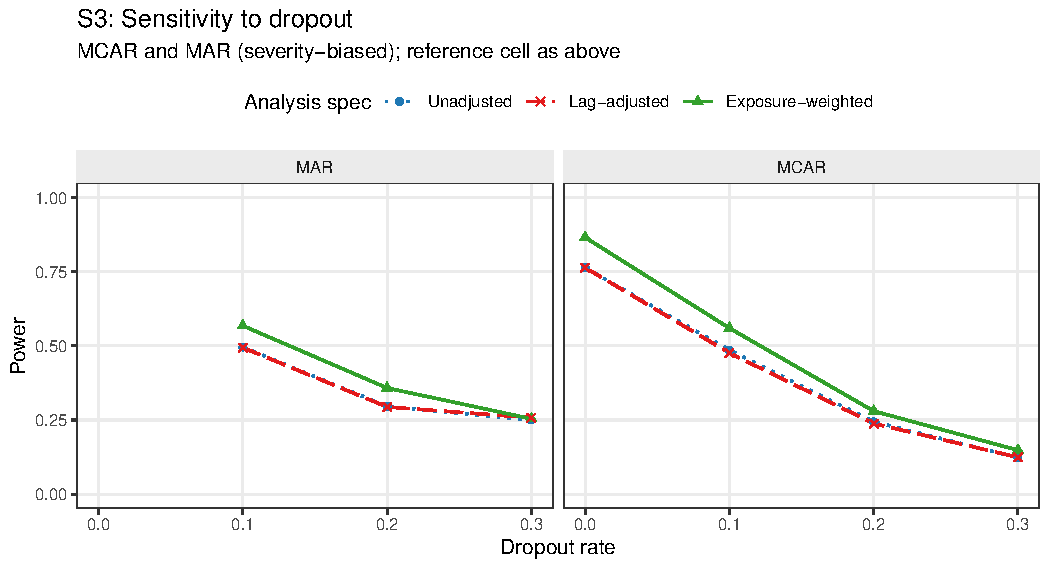
\includegraphics[width=0.8\linewidth]{../../figures/02xs-sens-S3} \caption{Power at dropout rates $\in \{0, 0.1, 0.2, 0.3\}$ under MCAR and MAR mechanisms.}\label{fig:fig-sens-s3}
\end{figure}

\begin{figure}
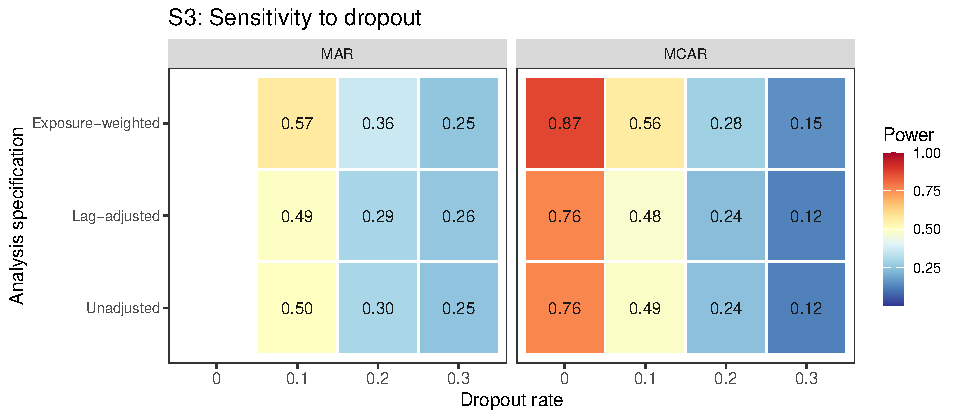
\includegraphics[width=0.8\linewidth]{../../figures/02xs-heatmap-sens-S3} \caption{Block S3: power by dropout rate and analysis specification, faceted by dropout mechanism, same data as the line plot above. The MAR arm has no $0\%$ cell (Section 3.7); it shares the MCAR reference cell.}\label{fig:fig-heatmap-sens-s3}
\end{figure}

\begin{figure}
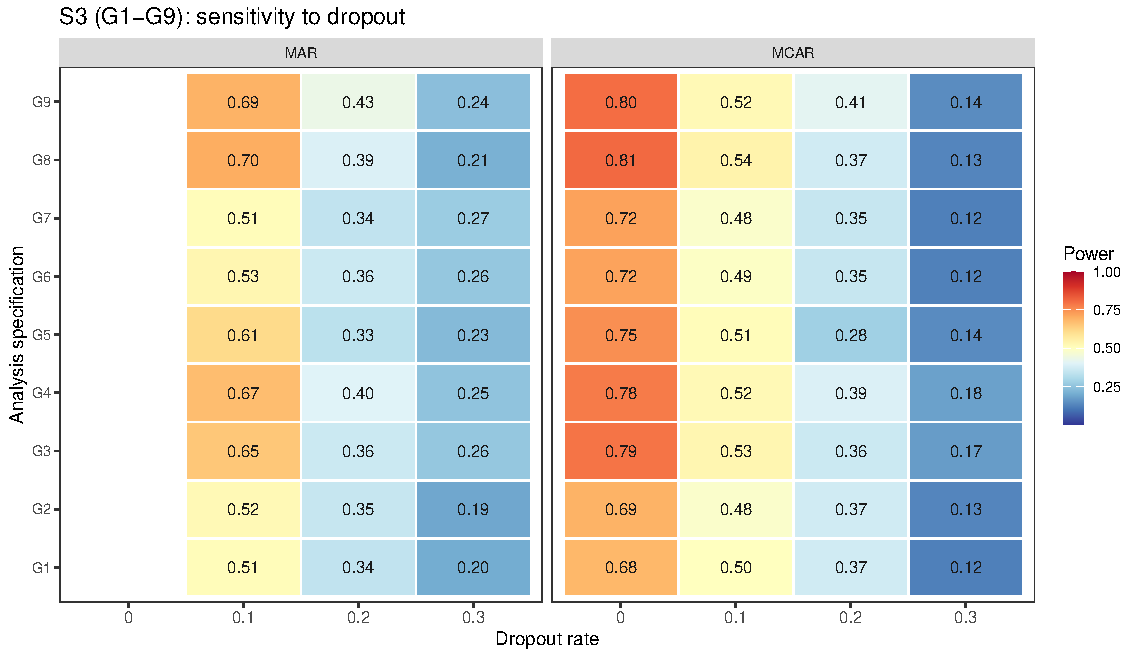
\includegraphics[width=0.9\linewidth]{../../figures/02xs-heatmap-sens-S3-g9} \caption{Block S3 extended to all nine G1-G9 specifications (preliminary $n_{sim} = 100$).}\label{fig:fig-heatmap-sens-s3-g9}
\end{figure}

\begin{itemize}
\tightlist
\item
  All three specifications lose power monotonically as dropout
  increases.
\item
  At the MCAR baseline (N=70, no dropout), Exposure-weighted gives
  \(0.866 \pm 0.015\) against \(0.764 \pm 0.019\) for the other two.
\item
  At 30\% MCAR dropout, all three collapse to \(0.122\) to \(0.148\).
\item
  The Exposure-weighted advantage narrows steadily as dropout
  worsens: about 0.10 absolute at zero dropout, 0.07 at 10\%, 0.04 at
  20\%, 0.03 at 30\% under MCAR, narrowing further under MAR at the
  highest rate.
\item
  Consistent with the advantage originating in the exposure-weighted
  contrast from off-drug observations, which contracts as those
  observations are preferentially lost.
\item
  The advantage is preserved at dropout of 20\% or below.
\item
  Lag-adjusted again tracks Unadjusted throughout (largest
  discrepancy 0.010).
\end{itemize}

\subsubsection{S4: biomarker-moderation effect-size curve}\label{s4-biomarker-moderation-effect-size-curve}

\begin{itemize}
\tightlist
\item
  The power curve is sigmoidal for all three original specifications
  across \(c_{bm} \in \{0, 0.10, 0.20, 0.30, 0.45, 0.60\}\), saturating
  once \(c_{bm} \geq 0.45\).
\item
  The Exposure-weighted advantage over the unadjusted benchmark is
  largest at intermediate effect sizes (\(+0.10\) absolute at
  \(c_{bm}=0.45\)), shrinking as all three approach the ceiling.
\item
  Implication: the advantage matters most for trials targeting a
  moderate biomarker-treatment interaction.
\item
  Full curve and nine-specification extension: Supplement, Section
  S4.
\end{itemize}

\subsubsection{S7: alternative-paradigm specifications}\label{s7-alternative-paradigm-specifications}

\begin{itemize}
\tightlist
\item
  An earlier version of this block tested two carryover terms crossed
  with the biomarker:

  \begin{itemize}
  \tightlist
  \item
    \texttt{E5}: \(\text{Sx} \sim bm + t + D_{it} + \text{bm:}D_{it} +
    L_{it} + \text{bm:}L_{it}\).
  \item
    \texttt{E6}: \(\text{Sx} \sim bm + t + D_{it} + \text{bm:}D_{it} +
    t_{sd} + \text{bm:}t_{sd}\).
  \end{itemize}
\item
  Motivated by Section 4.1's observation that a nuisance-main-effect
  carryover term cannot repair the interaction's attenuation.
\item
  Both underperformed Unadjusted at every cell examined, evaluated by
  a joint 2-df Wald test (each adds a second interaction
  coefficient).
\item
  Traced to a structural cause (Section 4.6): the DGP has a single
  true decay parameter, so a second, DGP-unmotivated interaction
  coefficient mostly adds estimation noise.
\item
  \texttt{E5}/\texttt{E6} were replaced by \texttt{G4} (AIC-selected half-life) and \texttt{G5}
  (paired-difference regression), both single-coefficient tests,
  unlike \texttt{E5}/\texttt{E6}.
\end{itemize}

\begin{table}
\centering
\caption{\label{tab:tab-s7}Block S7: all five G1-G5 specifications at the
    reference cell (Hybrid, $N = 70$, $c_{bm} = 0.45$,
    $t_{1/2} = 1.0$, exponential DGP, $n_{sim} = 500$, all
    replicates converged). G4 targets bm:Dbc at the AIC-selected
    half-life (candidate grid 0.25, 0.5, 1.0, 2.0); G5 targets the
    slope of the patient-level diff~bm regression. Neither is the
    same estimand as bm:Db (G1/G2), so only power is comparable
    across rows. Mean selected t1/2 is the average AIC-chosen
    half-life for G4 across replicates, against a true half-life of
    1.0.}
\centering
\resizebox{\ifdim\width>\linewidth\linewidth\else\width\fi}{!}{
\begin{tabular}[t]{lll}
\toprule
Specification & Power (MCSE) & Mean selected t1/2\\
\midrule
G1: Unadjusted & 0.748 (0.019) & --\\
G2: Lag-adjusted & 0.748 (0.019) & --\\
G3: Exposure-weighted & 0.826 (0.017) & --\\
G4: AIC-selected t1/2 & 0.832 (0.017) & 1.31\\
G5: Paired-difference & 0.804 (0.018) & --\\
\bottomrule
\end{tabular}}
\end{table}

\begin{figure}
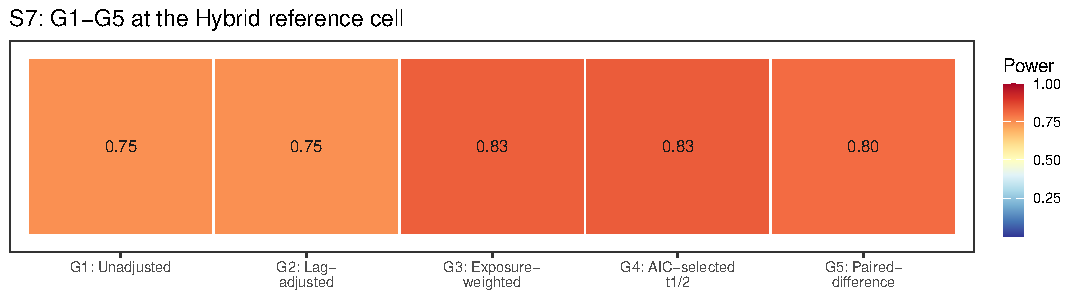
\includegraphics[width=0.75\linewidth]{../../figures/02xs-heatmap-sens-S7} \caption{Block S7: power by analysis specification, same figures as the table above.}\label{fig:fig-heatmap-sens-s7}
\end{figure}

\begin{itemize}
\tightlist
\item
  Table \ref{tab:tab-s7} gives a genuinely different result from the
  retired \texttt{E5}/\texttt{E6} comparison: \texttt{G4} and \texttt{G5} both beat Unadjusted at
  this cell, and \texttt{G4} edges out \texttt{G3} (Exposure-weighted) too.
\item
  Ranking at this cell: \texttt{G4} leads (\(0.832\)), \texttt{G3} follows (\(0.826\)),
  then \texttt{G5} (\(0.804\)), then \texttt{G1}/\texttt{G2} tied at the back (\(0.748\) each,
  the Section 3.4 null replicated once more).
\item
  \texttt{G4}'s AIC selection is imperfect but usefully informative: mean
  selected half-life is \(1.31\) weeks against a true value of \(1.0\),
  with the selection distribution concentrating on the true value and
  its immediate neighbor (a computed percentage choosing \(1.0\) or
  \(2.0\) weeks, per the inline \texttt{r} computation in the source). This is
  close enough to the truth that \texttt{G4} slightly exceeds \texttt{G3}'s own
  oracle-half-life power at this cell.
\item
  Notable result in \texttt{G5}: it discards the repeated-measures structure,
  correlation model, and any carryover representation entirely, and
  still beats \texttt{G1}/\texttt{G2}, echoing Senn, Julious and Araujo's\textsuperscript{\citeproc{ref-senn2014four}{7}} finding that simplicity is not obviously costly
  for N-of-1 treatment-effect estimation.
\item
  These results should not be read as general: Block S9, next, tests
  whether the ranking survives a different trial design, and it does
  not for every specification equally.
\end{itemize}

\subsubsection{S8: architecture sensitivity of the specification ranking}\label{s8-architecture-sensitivity-of-the-specification-ranking}

\begin{itemize}
\tightlist
\item
  Every result reported to this point (Tier 1 and blocks S1-S7 alike)
  is restricted to Architecture B (covariance moderation), the
  manuscript's stated scope (Section 2.3).
\item
  Block S8 asks a narrower question than a full architecture
  comparison (the purpose of the companion manuscript\textsuperscript{\citeproc{ref-pmsimstats_dgp_architectures2026}{3}}): does the specification
  ranking established under Architecture B hold under Architecture A
  (mean moderation), or is the choice of carryover representation
  itself architecture-dependent?
\item
  Refits the five S7 specifications at the same reference cell under
  both architectures, at three half-lives (\(t_{1/2} \in \{0, 0.5,
  1.0\}\)).
\item
  The S7 result (\texttt{G4}/\texttt{G5} both beating \texttt{G1}) turns out to be
  architecture-specific, joining Exposure-weighted in a pattern that
  grows with carryover severity rather than switching on at a
  threshold.
\item
  Under Architecture B at \(t_{1/2}=1.0\): \texttt{G4} leads (\(0.850\)), ahead
  of \texttt{G5} (\(0.842\)), \texttt{G3} (\(0.836\)), and \texttt{G1}/\texttt{G2} (\(0.760\)).
\item
  Under Architecture A the pattern reverses for \texttt{G4} and \texttt{G3} alike:
  \texttt{G1}/\texttt{G2} lead (\(0.972\)/\(0.976\)), \texttt{G5} trails only slightly
  (\(0.964\)), \texttt{G3} (\(0.946\)) and \texttt{G4} (\(0.950\)) trail by 2 to 3
  points -- a real, if modest, reversal.
\item
  Matches the archived full-scope drafts' finding that
  Exposure-weighted is marginally dominated under mean moderation
  (Section 4.6); \texttt{G4} inherits the same sensitivity, sharing
  Exposure-weighted's formula.
\item
  \texttt{G5} is comparatively more robust to architecture, never reversing
  to a large disadvantage either way.
\item
  Lag-adjusted (\texttt{G2}) remains statistically indistinguishable from
  Unadjusted (\texttt{G1}) under both architectures at every half-life,
  extending Section 3.4's clean null to Architecture A as well.
\item
  The manuscript's one specification recommendation (exposure
  weighting in Hybrid/OL+BDC) is therefore conditional on
  Architecture B and grows more important as carryover worsens; the
  same qualification now extends to \texttt{G4}.
\item
  Full cell-by-cell detail, table, and both architecture panels:
  Supplement, Section S8.
\end{itemize}

\subsubsection{S9: does the reference-cell ranking survive under CO?}\label{s9-does-the-reference-cell-ranking-survive-under-co}

\begin{itemize}
\tightlist
\item
  Blocks S7-S8 found \texttt{G4} and \texttt{G5} both beat Unadjusted at the
  Hybrid reference cell under Architecture B, with \texttt{G4} slightly
  exceeding Exposure-weighted (\texttt{G3}) itself.
\item
  Block S9 asks whether that ranking is specific to Hybrid's short,
  compressed washout, refitting all five G1-G5 specifications under
  CO (off-drug arm spanning 2.5 to 20 weeks post-discontinuation,
  Section 2.2) at two true half-lives.
\end{itemize}

\begin{figure}
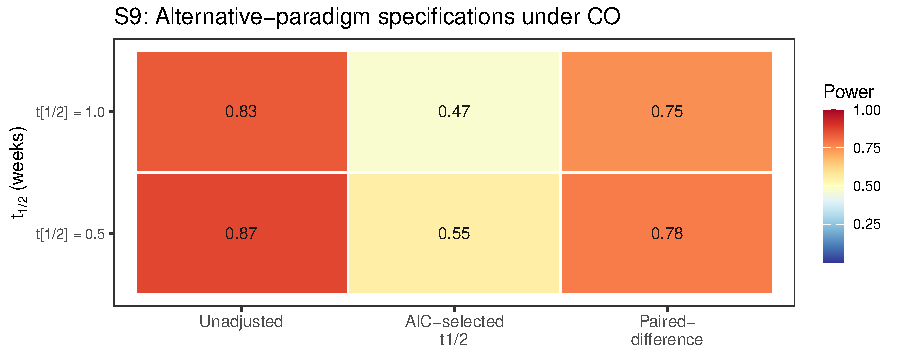
\includegraphics[width=0.8\linewidth]{../../figures/02xs-heatmap-sens-S9} \caption{Block S9: power under the CO design at two true half-lives, all five G1-G5 specifications.}\label{fig:fig-heatmap-sens-s9}
\end{figure}

\begin{itemize}
\tightlist
\item
  It is not design-general, and including \texttt{G3} changes the diagnosis
  reached from \texttt{G4} alone.
\item
  At \(t_{1/2}=1.0\): \texttt{G1}/\texttt{G2} lead (\(0.834\)/\(0.838\)); \texttt{G5} trails
  moderately (\(0.750\)); \texttt{G3} and \texttt{G4} both collapse, to \(0.482\) and
  \(0.474\) respectively, statistically indistinguishable from each
  other (gap \(0.008\), well under one MCSE).
\item
  At \(t_{1/2}=0.5\) the same pattern holds (\(0.866\)/\(0.864\) for
  \texttt{G1}/\texttt{G2}, \(0.778\) for \texttt{G5}, \(0.546\)/\(0.552\) for \texttt{G3}/\texttt{G4}, again
  indistinguishable).
\item
  Because \texttt{G3} uses the \emph{true} half-life (not estimated), its
  near-identical collapse shows \texttt{G4}'s CO failure is inherited almost
  entirely from Exposure-weighted's own established weakness under
  this design (Section 3.4: \(0.488\) versus \(0.830\)), not created by
  the AIC-selection step.
\item
  A separately confirmed pathology exists in the selection step
  itself: it concentrates overwhelmingly on the largest candidate
  half-life (\(2.0\) weeks, chosen in 483 of 500 replicates at
  \(t_{1/2}=1.0\), 435 of 500 at \(t_{1/2}=0.5\), regardless of true
  half-life), consistent with a weakly informative likelihood surface
  when off-drug occasions are few and widely spaced.
\item
  But that mis-selection costs \texttt{G4} essentially nothing beyond what
  \texttt{G3} already loses under CO with the correct half-life in hand; the
  dominant story is the continuous decayed predictor's mismatch with
  CO's design generally, with AIC selection an identified but
  practically minor addition.
\item
  \texttt{G5}'s milder reversal has no comparable mechanical explanation: it
  reflects that CO's own within-subject contrast already captures
  most of the signal a between-patient paired-difference regression
  is built to extract, so discarding the repeated-measures structure
  costs more under CO than under Hybrid.
\item
  None of \texttt{G3}, \texttt{G4}, \texttt{G5}'s Hybrid-cell behavior is design-general;
  the design-specific guidance in Section 4.5 should be read
  accordingly: \texttt{G3}/\texttt{G4} should not be used under CO regardless of
  whether the half-life is assumed or estimated.
\end{itemize}

\subsubsection{S10: does a CR2 correction change the ranking among G1-G9?}\label{s10-does-a-cr2-correction-change-the-ranking-among-g1-g9}

\begin{itemize}
\tightlist
\item
  Section 3.6 (Block S6) showed the model-based interaction test is
  mildly conservative and CR2 recovers two to five points of power
  without disturbing the ranking among \texttt{G1}, \texttt{G3}, \texttt{G2}; that
  correction had not been applied to \texttt{G4} or \texttt{G5}.
\item
  This block asks whether CR2 helps \texttt{G4} and \texttt{G1}/\texttt{G2} the way it
  already helps \texttt{G3}, and whether it changes which specification
  leads at the Hybrid, Architecture B reference cell.
\item
  Uses the compact \texttt{G1}-\texttt{G9} naming layer: \texttt{G6}-\texttt{G9} cross CR2 with
  \texttt{G1}, \texttt{G2}, \texttt{G4}, \texttt{G3}. \texttt{G5} has no CR2 variant (paired-difference
  regression collapses to one row per patient before fitting, leaving
  no cluster structure for CR2 to correct).
\item
  CR2 helps every specification it was applied to:

  \begin{itemize}
  \tightlist
  \item
    \texttt{G1}/\texttt{G2} (both \(0.748\) model-based) rise to \texttt{G6} \(0.776\) and
    \texttt{G7} \(0.764\).
  \item
    The ranking among the five base specifications is unchanged by
    these gains, since \texttt{G1}/\texttt{G2} remain well below \texttt{G3}-\texttt{G5}
    regardless.
  \end{itemize}
\item
  What does change the ranking: \texttt{G9} -- CR2 lifts \texttt{G4} (\(0.832\)
  model-based) to \(0.870\), a \(3.8\)-point gain, the largest CR2
  correction observed anywhere in this manuscript, enough for \texttt{G9}
  to overtake every other specification tested, including \texttt{G8}
  (\(0.863\)).
\item
  This did not come with a Type I error cost (checked directly in
  Section S11 of the Supplement): every replicate converged under
  \texttt{G9}, and the power gain is consistent with CR2 correcting real
  conservatism rather than papering over a different problem.
\item
  Full detail, reference-cell table, and heatmap: Supplement, Section
  S10.
\end{itemize}

\subsubsection{S11: is G4's Type I error controlled?}\label{s11-is-g4s-type-i-error-controlled}

\begin{itemize}
\tightlist
\item
  \texttt{G4} selects its half-life by AIC then tests the interaction
  coefficient from the selected model, a post-selection inference
  problem: the same data drive both selection and test, which can in
  principle inflate Type I error beyond nominal.
\item
  Block S11 checks this directly, refitting \texttt{G1}-\texttt{G5} and \texttt{G9} at the
  null (\(c_{bm}=0\)) at the Hybrid reference cell, with \(n_{sim}=2000\)
  for tighter precision on a rate expected near \(0.05\).
\item
  The concern does not materialize: \texttt{G4}'s Type I error is \(0.038\),
  conservative and in the same range as \texttt{G1}-\texttt{G3} (\(0.034\)-\(0.036\)),
  not inflated by the selection step.
\item
  \texttt{G9} (\texttt{G4}+CR2) is \(0.052\), indistinguishable from nominal \(0.05\).
\item
  Read together with Section 3.6's power results: \texttt{G9}'s status as
  the best-performing specification (Section 3.7, Block S10) is not
  an artifact of an uncontrolled test -- it wins on power while
  holding Type I error at nominal, the same standard \texttt{G3}+CR2 (\texttt{G8})
  is held to.
\item
  This does not generalize beyond the single cell tested.
\item
  Full detail and heatmap: Supplement, Section S11.
\end{itemize}

\textbf{Section summary:}

\begin{itemize}
\tightlist
\item
  Nine Tier 2 sensitivity blocks (S1-S4, S7-S11), plus S6 (CR2
  recalibration) and an out-of-scope S5, perturb one axis at a time
  around the Hybrid/\(N\)=70/\(c_{bm}\)=0.45/exponential/\(t_{1/2}\)=1.0
  reference cell.
\item
  Robustness holds for the core Exposure-weighted advantage under
  autocorrelation (S1) and moderate half-life mis-assumption (S2),
  narrows under dropout (S3) and at extreme effect sizes (S4).
\item
  The alternative-paradigm specifications \texttt{G4} and \texttt{G5} (replacing
  the structurally flawed \texttt{E5}/\texttt{E6}) beat Exposure-weighted at the
  Hybrid Architecture-B reference cell (S7), but both results reverse
  or collapse under Architecture A (S8) and under the CO design (S9),
  so neither generalizes beyond that single cell type.
\item
  CR2 correction helps every specification, most dramatically \texttt{G4}
  (yielding \texttt{G9}, the single best-performing specification found
  anywhere in this manuscript), without inflating Type I error (S10,
  S11) -- but again validated at only one cell.
\end{itemize}

\subsection{A higher-precision check}\label{a-higher-precision-check}

\begin{itemize}
\tightlist
\item
  Because a number of the Tier 1 gaps are small, a focused 24-cell
  grid (OL+BDC design, \(N \in \{35, 70\}\), true half-life \(\in \{0.5,
  1.0\}\)) was rerun at 600 trials per cell, all converging.
\item
  Specifications were compared with a paired McNemar test,
  considerably more sensitive than an independent-groups comparison
  since all three are fit to the same trials.
\item
  Type I error across the twelve null cells fell in \([0.003, 0.053]\),
  so nominal alpha holds.
\item
  Paired McNemar tests place Exposure-weighted ahead of the unadjusted
  benchmark at all four alternative cells, by \(+2.3\) to \(+13.7\)
  percentage points.
\item
  Largest gap at the highest-leverage cell (\(N=70\), true
  \(t_{1/2}=1.0\) weeks, \(p = 6.6 \times 10^{-17}\)), with \(p \leq
  0.015\) at the remaining three -- a sharper confirmation than the
  Tier 1 grid alone provides.
\item
  One scope caveat governs the rerun's third arm: it was produced by
  the package's \texttt{lme\_analysis()} routine, whose carryover option
  appends time since discontinuation as a linear main effect rather
  than the lagged indicator \(L_{it}\) used in the Tier 1 grid; it is
  therefore \textbf{not} the Lag-adjusted specification of Section 2.4 and
  is not reported as such here.
\item
  That alternative remains a reasonable specification not yet
  evaluated (Section 4.6).
\end{itemize}

\textbf{Section summary:}

\begin{itemize}
\tightlist
\item
  A higher-precision, paired-McNemar rerun (600 trials/cell, 24
  cells, OL+BDC only) confirms Exposure-weighted's advantage with
  much sharper statistical significance than the Tier 1 grid alone,
  while flagging that its third-arm comparator differs subtly from
  the manuscript's own Lag-adjusted definition.
\end{itemize}

\section{Discussion}\label{discussion}

\subsection{The lagged-treatment term does no work}\label{the-lagged-treatment-term-does-no-work}

\begin{itemize}
\tightlist
\item
  The clearest result of this study is a negative one: adding the
  classical lagged-treatment indicator changed nothing measurable,
  anywhere in the grid.
\item
  Across all 216 cells, mean power difference against the unadjusted
  benchmark was 0.003 against an MCSE of 0.018; bias, MSE, coverage
  agreed to three decimal places, in every sensitivity block and all
  five cluster-robust stress cells under both inference procedures.
\item
  The strength of this conclusion rests on the design rather than
  grid size: the two specifications estimate the same coefficient,
  are fitted to the same simulated datasets under common random
  numbers, and differ by exactly one term.
\item
  No confounding from a change of estimand, Monte Carlo variation
  between arms, or differential test size (both conservative to the
  same degree, Section 3.6); what is left is the term itself, and it
  contributed nothing.
\item
  Mechanism follows from where the term sits: carryover damages the
  interaction test on two fronts (Section 1) -- attenuates the
  coefficient (contaminated occasions coded as drug-free) and
  inflates residual variance (heterogeneity the model does not
  represent).
\item
  The lagged indicator enters only as a nuisance main effect with no
  \(\text{bm:}L_{it}\) product, so the tested interaction remains
  \(\text{bm:}D_{it}\) and the attenuation is untouched.
\item
  It can in principle absorb some of the residual-variance effect,
  but evidently absorbs too little to matter: it marks a single
  occasion per randomization path and is constant thereafter, unable
  to describe a graded decline across a two- to four-occasion
  washout.
\item
  A targeted check on a more capable, elapsed-time-indexed nuisance
  term (\texttt{Sx\ \textasciitilde{}\ bm\ +\ t\ +\ Db\ +\ bm:Db\ +\ tsd}, the ``washout-adjusted''
  specification \texttt{E4} from the reference implementation) was run
  across the three designs at true half-lives 0.5 and 1.0 weeks
  (\(N=70\), \(c_{bm}=0.45\), exponential DGP, 500 replicates):

  \begin{itemize}
  \tightlist
  \item
    Type I error at nominal for both (mean 0.050 vs 0.045).
  \item
    Power exceeds the benchmark in all six cells by a mean of 1.3
    points (sign test \(p=0.031\)).
  \item
    Reaches significance under crossover at both half-lives (\(+1.8\),
    \(p=0.008\); \(+2.2\), \(p=0.003\)) and OL+BDC at the longer half-life
    (\(+2.2\), \(p=0.015\)), but not Hybrid (\(+1.0\), \(p=0.27\)).
  \item
    Mechanism matches Section 2.4's prediction: point estimates are
    unchanged (nothing about attenuation is repaired), the entire
    effect runs through the standard error, which only a long enough
    washout gives it something to describe.
  \item
    Crossover places off-drug occasions 2.5 to 10 weeks post-
    discontinuation, against one to two weeks for Hybrid.
  \item
    Practical ceiling on any carryover nuisance term is therefore
    about two percentage points, only in long-washout designs,
    against the nine to eleven points exposure weighting delivers
    where it works.
  \item
    This check covers only the exponential DGP at a single \(N\) and
    effect size, so it is a probe rather than a fourth arm; it shares
    every specification's structural limitation of entering carryover
    as a main effect only (Section 4.6).
  \end{itemize}
\item
  Practical implication: a carryover nuisance term of either form
  should not be expected to recover meaningful power lost to
  carryover, and reporting one does not constitute an effective
  adjustment for it.
\end{itemize}

\textbf{Section summary:}

\begin{itemize}
\tightlist
\item
  Both the classical lagged-treatment term and a more capable
  elapsed-time nuisance term (E4) fail to meaningfully repair the
  interaction test's power loss from carryover, because a nuisance
  main effect cannot touch the attenuation mechanism, only (weakly)
  the residual-variance mechanism.
\item
  The practical ceiling on any nuisance-term-only carryover
  adjustment is about two percentage points, in long-washout designs
  only, versus the nine-to-eleven-point gain from exposure weighting
  where it works.
\end{itemize}

\subsection{The exposure-weighted advantage, and where it fails}\label{the-exposure-weighted-advantage-and-where-it-fails}

\begin{itemize}
\tightlist
\item
  At its best cell (Hybrid, \(N=70\), \(c_{bm}=0.45\), \(t_{1/2}=1.0\)), the
  exposure-weighted predictor exceeds the unadjusted benchmark by
  about 10 points of power (0.860 versus 0.766, roughly five MCSEs,
  not attributable to chance), confirmed at all four cells of the
  Section 3.8 high-precision rerun.
\item
  Under crossover it performs considerably worse (0.488 versus
  0.830).
\item
  Proposed mechanism: the within-subject correlation under crossover
  already carries most of the signal the decaying predictor was
  designed to recover, so it gains little there while its
  down-weighting of off-drug observations works against it.
\item
  The recommendation therefore holds only in the two non-crossover
  designs and should not be extended to a crossover trial, where the
  unadjusted binary indicator is materially better.
\item
  That the one specification addressing attenuation (Exposure-
  weighted) is also the only one to gain power, while the one
  addressing only residual variance (Lag-adjusted) gains nothing,
  suggests attenuation is the mechanism that matters here -- read as
  an interpretation consistent with the results, not a finding the
  design isolates directly.
\end{itemize}

\textbf{Section summary:}

\begin{itemize}
\tightlist
\item
  Exposure weighting's power advantage is substantial (\textasciitilde10 points) in
  Hybrid/OL+BDC designs but reverses under crossover, attributed to
  crossover's own within-subject correlation already capturing the
  signal the predictor targets.
\item
  The pattern (only the attenuation-addressing specification gains
  power) is offered as a consistent interpretation, not a directly
  isolated causal finding.
\end{itemize}

\subsection{What the robustness checks add}\label{what-the-robustness-checks-add}

\begin{itemize}
\tightlist
\item
  The Section 3.7 sensitivity blocks show the exposure-weighted
  advantage, where it exists, is not uniformly fragile but not
  unconditionally robust either:

  \begin{itemize}
  \tightlist
  \item
    Under incorrect decay-shape assumptions (Figure
    \ref{fig:fig-heatmap-mismatch}, Section 3.5), it widens on the
    light-tailed side and narrows to statistical insignificance on
    the heavy-tailed side, disappearing entirely at the two most
    extreme Weibull shapes examined (\(k=0.25\), \(0.5\)).
  \item
    It survives an incorrectly assumed half-life, short of a large
    over-assumption at a short true half-life (Block S2, Supplement
    Section S2).
  \item
    It holds its five- to eight-point lead across the autocorrelation
    range examined (Block S1, Supplement Section S1).
  \end{itemize}
\item
  Decay-shape mis-specification is therefore the one robustness axis
  examined here that can erode the advantage away entirely, rather
  than only narrowing it.
\item
  One caveat governs the Tier 1 figures throughout: outside Block S2,
  the analysis-side half-life is set equal to the data-generating
  one, granting Exposure-weighted an oracle no real analyst
  possesses, so its Tier 1 margins are upper bounds, and Block S2
  gives the more realistic figure.
\end{itemize}

\textbf{Section summary:}

\begin{itemize}
\tightlist
\item
  Robustness of the exposure-weighted advantage varies by axis:
  robust to autocorrelation and moderate half-life mis-assumption,
  fragile to decay-shape mis-specification (can vanish entirely at
  extreme shapes).
\item
  All Tier 1 figures outside Block S2 grant Exposure-weighted an
  oracle half-life, so those margins should be read as upper bounds.
\end{itemize}

\subsection{Dropout matters more than the method}\label{dropout-matters-more-than-the-method}

\begin{itemize}
\tightlist
\item
  The finding with the largest practical consequence concerns missing
  data, not carryover: when patients drop out (Figure
  \ref{fig:fig-sens-s3}), power collapses for all three
  specifications together, to between 0.12 and 0.25 at 30\% dropout,
  essentially indistinguishable.
\item
  No specification offers protection, since each can only organize
  whatever data remain.
\item
  MAR dropout is somewhat worse than MCAR, because the sickest
  patients, who carry the most signal, tend to leave first.
\item
  Retaining patients in the trial yields considerably more power than
  any choice among the three specifications ever could.
\end{itemize}

\textbf{Section summary:}

\begin{itemize}
\tightlist
\item
  Dropout is the single largest power lever in the study, dwarfing
  any effect of analysis-specification choice; no specification
  offers protection against it.
\end{itemize}

\subsection{What analysis is best in which situations, in practice}\label{what-analysis-is-best-in-which-situations-in-practice}

Collecting the findings above into a decision rule rather than a set
of pairwise comparisons:

\begin{itemize}
\tightlist
\item
  \textbf{Covariance moderation (Architecture B), Hybrid or OL+BDC
  design.} Use Exposure-weighted with a CR2 cluster-robust standard
  error.

  \begin{itemize}
  \tightlist
  \item
    The advantage holds under half-life mis-specification short of a
    large over-assumption (Section 3.7, Block S2), and across the
    autocorrelation range examined (Block S1).
  \item
    It holds and widens under decay-shape mis-specification on the
    light-tailed side, but narrows to statistical insignificance at
    the two most extreme heavy-tailed shapes examined (Section 3.5):
    this recommendation should not be read as holding under an
    arbitrarily heavy-tailed decay form.
  \item
    CR2 restores nominal Type I error without disturbing the ranking
    (Block S6, validated at \(N \in \{35, 70\}\) in the Hybrid design
    specifically; OL+BDC was not itself stress-tested under CR2).
  \item
    This remains the recommended default: it has been through the
    full robustness battery \texttt{G4}/\texttt{G5} have not (next point).
  \end{itemize}
\item
  \textbf{\texttt{G4} (AIC-selected half-life) and \texttt{G5} (paired-difference) are
  promising at this same cell, not yet validated defaults.}

  \begin{itemize}
  \tightlist
  \item
    Both beat Exposure-weighted itself at the Hybrid, Architecture B
    reference cell (Blocks S7-S8: \texttt{G4} \(0.850\), \texttt{G5} \(0.842\), \texttt{G3}
    \(0.836\), at \(t_{1/2}=1.0\)), and \texttt{G4} in particular removes the
    need to assume a half-life at all.
  \item
    Neither has been tested against decay-shape mis-specification,
    dropout, or under CR2 the way \texttt{G3} has, so this is grounds to
    investigate them further, not to displace the established
    default yet.
  \item
    Adding a CR2 correction to \texttt{G4} (\texttt{G9} in the nine-way naming
    layer) goes further still: at this same cell it outperforms every
    one of the other eight specifications, including \texttt{G3}+CR2, with
    no accompanying Type I error inflation (Section 3.7, Blocks
    S10-S11).
  \item
    This is the single best result anywhere in this manuscript, and
    also the least validated: it rests on one cell, with none of
    \texttt{G4}'s own robustness gaps yet closed.
  \end{itemize}
\item
  \textbf{Crossover (CO) design, any architecture.} Use Unadjusted.

  \begin{itemize}
  \tightlist
  \item
    Exposure-weighted is markedly worse under CO (Section 3.4), and
    Block S9 shows \texttt{G4} and \texttt{G5} fail here too, \texttt{G4} catastrophically.
  \item
    \texttt{G4}'s AIC half-life selection systematically drifts to the
    largest candidate in its grid under CO's sparse, widely spaced
    off-drug sampling (chosen in over 85\% of replicates regardless of
    true half-life), collapsing its power to roughly half of
    Unadjusted's; it should specifically be avoided under any design
    with few, widely spaced off-drug observations.
  \item
    \texttt{G5} also underperforms Unadjusted under CO, though far more
    mildly.
  \item
    The classical lagged-treatment remedy adds nothing here either,
    including in the one design where its washout is long enough to
    give it a chance (Section 4.1).
  \end{itemize}
\item
  \textbf{Architecture uncertain, or known to be mean moderation
  (Architecture A).} Use Unadjusted or Lag-adjusted, not
  Exposure-weighted or \texttt{G4}.

  \begin{itemize}
  \tightlist
  \item
    Both specifications' advantage under covariance moderation
    reverses, marginally, under mean moderation (Block S8).
  \item
    \texttt{G5} is the one specification whose performance does not depend
    much on which architecture generated the data (small under B,
    smaller under A), but it has been tested at only one design and
    reference cell outside the Hybrid comparison (Block S9).
  \end{itemize}
\item
  \textbf{Never rely on Lag-adjusted as a carryover remedy.}

  \begin{itemize}
  \tightlist
  \item
    It is statistically indistinguishable from Unadjusted everywhere
    tested in this manuscript, Tier 1 and every Tier 2 block alike
    (Section 4.1).
  \item
    If a reviewer or protocol expects some carryover term to be
    present, including it costs nothing measurable, but it should not
    be reported as having adjusted for carryover.
  \end{itemize}
\item
  \textbf{Minimize dropout before optimizing specification choice.}

  \begin{itemize}
  \tightlist
  \item
    It is the single largest lever in the entire grid (Section 4.4),
    and no specification, including \texttt{G4}/\texttt{G5}, has been shown to
    offer any protection against it; their behavior under dropout is
    untested.
  \end{itemize}
\end{itemize}

\subsubsection{Why G4 and G5 succeed at Hybrid but fail under CO}\label{why-g4-and-g5-succeed-at-hybrid-but-fail-under-co}

\begin{itemize}
\tightlist
\item
  Both new specifications' Hybrid, Architecture B advantage
  evaporates under the CO design (Block S9), for two different,
  design-specific reasons rather than a shared structural flaw of the
  kind that sank \texttt{E5}/\texttt{E6} (Section 4.6).
\item
  \texttt{G4}'s failure is mechanical: with only a few, widely spaced
  off-drug occasions, the likelihood surface across candidate
  half-lives is weakly informative, and AIC selection drifts to the
  boundary of its candidate grid rather than locating the true value,
  systematically overestimating the half-life.
\item
  Section 3.7's S2 block already showed over-assumption is the more
  damaging direction of half-life error when the half-life is fixed
  by the analyst; under CO, \texttt{G4} reproduces that same damaging error
  through the estimation procedure itself, on nearly every replicate.
\item
  Concrete, testable prediction: \texttt{G4} should be reliable whenever a
  design gives several off-drug occasions across a graded range of
  elapsed time (as Hybrid does despite its short overall washout),
  and unreliable whenever off-drug sampling is sparse, however long
  the washout runs in calendar time.
\item
  \texttt{G5}'s failure has no comparable mechanical account and is milder:
  the most plausible explanation is that CO's own within-subject
  contrast (Section 3.4) already carries most of the signal a
  between-patient paired-difference regression is built to extract,
  so discarding the repeated-measures and correlation structure costs
  more under CO than under Hybrid, where that structure is doing more
  work. This was not tested directly and would require comparing
  \texttt{G5} against the within-cell decomposition of \texttt{G3}'s advantage to
  confirm.
\item
  Two implications follow:

  \begin{itemize}
  \tightlist
  \item
    These results reinforce rather than undercut the earlier
    \texttt{E5}/\texttt{E6} diagnosis (Section 4.6): the more fundamental unresolved
    question is not which design an alternative specification is
    tested under, but whether the underlying DGP rewards that
    specification's added structure at all -- neither \texttt{G4} nor \texttt{G5}
    was tested against a DGP built to favor them specifically.
  \item
    The practical recommendation is narrower than ``estimate the
    half-life'' or ``use a simpler method'': both \texttt{G4} and \texttt{G5} are
    candidates worth validating further within the Hybrid/OL+BDC,
    Architecture B cell where this manuscript's other recommendations
    already concentrate, not general-purpose replacements for
    Exposure-weighted or Unadjusted.
  \end{itemize}
\end{itemize}

\textbf{Section summary:}

\begin{itemize}
\tightlist
\item
  The manuscript's practical decision rule is design- and
  architecture-conditional: Exposure-weighted+CR2 for Hybrid/OL+BDC
  under Architecture B; Unadjusted for crossover or uncertain/
  Architecture A; Lag-adjusted never recommended as a standalone
  remedy; dropout minimization takes priority over specification
  choice.
\item
  \texttt{G4}/\texttt{G9} and \texttt{G5} are flagged as promising but under-validated,
  with \texttt{G4}'s CO failure traced to a mechanical AIC boundary-drift
  problem under sparse off-drug sampling, and \texttt{G5}'s milder CO
  failure attributed (untested) to CO's within-subject contrast
  already capturing the signal the paired-difference approach targets.
\end{itemize}

\subsection{Scope, related work, and limits}\label{scope-related-work-and-limits}

\begin{itemize}
\tightlist
\item
  This manuscript deliberately narrows the full-scope grid to the
  covariance-moderation architecture and non-linear decay forms, in
  the interest of a self-contained evaluation of manageable length.
\item
  The archived full-scope drafts (\texttt{archive/report.Rmd},
  \texttt{archive/report-slim.Rmd}) show the exposure-weighted advantage
  documented here does not carry over to mean moderation, where
  Exposure-weighted is marginally dominated in every design examined;
  readers needing that cross-architecture comparison should consult
  those drafts rather than extrapolate from this one.
\item
  Establishing what the originally published power values (Section
  3.3) were computed under remains outstanding work.
\item
  The crossover tradition surveyed by Jones and Kenward\textsuperscript{\citeproc{ref-jones2014crossover}{4}} would lead one to expect a shape-free
  lagged term to outperform a parametric predictor once the decay
  shape is mis-specified; results here do not support that
  expectation over the range examined, for two reasons:

  \begin{itemize}
  \tightlist
  \item
    The exposure-weighted penalty for an incorrect half-life is too
    small to be overtaken (Section 3.7).
  \item
    More fundamentally, the lagged term does not improve on ignoring
    carryover at all (Section 4.1), leaving no advantage for
    decay-shape mis-specification to erode.
  \end{itemize}
\item
  One adjacent specification bounds the negative result of Section
  4.1: every carryover term considered there (lagged and
  washout-adjusted alike) enters as a nuisance main effect with no
  product against the biomarker, so the finding is that a carryover
  \emph{main effect} does not recover the attenuated signal, not that no
  shape-free specification can.
\item
  The natural candidate not yet tested is a carryover term interacted
  with the biomarker, either \texttt{Sx\ \textasciitilde{}\ bm\ +\ t\ +\ Db\ +\ bm:Db\ +\ L\ +\ bm:L} or
  its washout-adjusted counterpart with \texttt{bm:tsd}, letting the
  biomarker effect decline across the washout without committing to a
  rate.
\item
  An earlier version of Block S7 tested exactly these two
  specifications and found a clean negative result at every cell
  examined, traced to a structural cause: the DGP has a single true
  decay parameter, so a second, interacted carryover coefficient adds
  estimation noise without a corresponding signal to recover.
\item
  They were replaced by \texttt{G4} (AIC-selected half-life) and \texttt{G5} (a
  paired-difference regression with no carryover representation at
  all), addressing the same open problem (unknown decay half-life)
  from different angles.
\item
  Both beat Unadjusted at the Hybrid, Architecture B reference cell,
  \texttt{G4} even edging out Exposure-weighted itself (Block S7); neither
  survives a change of trial design or architecture (Blocks S8-S9).
\item
  \texttt{G4}'s AIC selection fails specifically under sparse off-drug
  sampling (Section 4.5); \texttt{G5}'s advantage appears to depend on the
  repeated-measures structure it discards being otherwise underused,
  which is design-dependent.
\item
  Block S8 shows the Lag-adjusted null of Section 3.4 replicates
  under Architecture A, so it is not an artifact specific to
  covariance moderation. Exposure-weighted's advantage, and now
  \texttt{G4}'s, are architecture-sensitive, reversing in direction (though
  not substantially) under Architecture A (Section 3.7, Block S8).
\item
  Three further N-of-1 analysis approaches sit outside the G1-G9
  family and are not evaluated here, each requiring substantial
  independent methodological development rather than a drop-in
  specification within the existing pipeline:

  \begin{itemize}
  \tightlist
  \item
    Tang and Landes\textsuperscript{\citeproc{ref-tang2020ttests}{10}}: formula-based \(t\)-tests
    correcting a single-subject paired-difference test's SE and
    degrees of freedom for an estimated first-order serial
    correlation -- the natural refinement \texttt{G5} lacks (\texttt{G5} discards
    within-patient correlation entirely). Their tests have no
    biomarker-moderation term, and would need a \texttt{diff\ \textasciitilde{}\ bm} extension
    with a serial-correlation-aware variance to enter this
    comparison.
  \item
    Schmid and Yang\textsuperscript{\citeproc{ref-schmid2022bayesian}{11}}: a Bayesian hierarchical
    alternative to the frequentist mixed-model/sandwich-estimator
    family spanning \texttt{G1}-\texttt{G9}, with partial pooling of individual-
    level treatment-effect, trend, and autocorrelation parameters
    across patients; they note carryover is tractable only in
    aggregated, multi-individual analyses like this one, but a
    biomarker-moderation extension of their model is a separate
    undertaking.
  \item
    Daza\textsuperscript{\citeproc{ref-daza2018causal}{12}}: frames N-of-1 inference as a
    counterfactual, time-varying-treatment problem, estimated via
    g-computation or inverse-probability weighting -- a structurally
    different paradigm from \texttt{G1}-\texttt{G9}'s explicit exponential-decay or
    lag covariates, treating carryover as confounding to be
    controlled rather than a predictor to be modeled.
  \end{itemize}
\item
  None of the three is a candidate for a tenth specification within
  this manuscript's scope, but each identifies a direction future
  work on this estimand should consider.
\item
  Two further limitations bound what can be concluded:

  \begin{itemize}
  \tightlist
  \item
    The numbers presented come from a single parameter set calibrated
    to a prazosin and PTSD trajectory, so absolute power values
    should be read as illustrative, and the ranking (itself
    conditional on trial design) as the more portable result.
  \item
    The sensitivity checks vary one factor at a time and can
    therefore miss genuine interactions between factors (e.g.,
    between high autocorrelation and heavy dropout); the one joint
    check available (Block S5 in the full-scope manuscript) revealed
    no such interaction.
  \end{itemize}
\end{itemize}

\textbf{Section summary:}

\begin{itemize}
\tightlist
\item
  This manuscript is a deliberately narrowed slice of a larger
  full-scope study; the archived drafts remain the authority on mean
  moderation and should be consulted before generalizing beyond
  covariance moderation.
\item
  The crossover literature's expectation that a shape-free lagged
  term would outperform a parametric predictor under decay-shape
  mis-specification is not supported here, because the lagged term
  fails even without mis-specification.
\item
  Three substantial alternative N-of-1 analysis paradigms (serial-
  correlation-corrected paired tests, Bayesian hierarchical models,
  counterfactual/causal-inference framing) remain outside this
  manuscript's scope and are flagged as future-work directions, not
  rejected findings.
\item
  Conclusions rest on a single calibrated parameter set and
  one-factor-at-a-time sensitivity checks, so absolute power values
  are illustrative and possible factor interactions beyond the one
  jointly checked (autocorrelation x dropout, no interaction found)
  remain unexamined.
\end{itemize}

\section{Conclusions}\label{conclusions}

\begin{enumerate}
\def\labelenumi{\arabic{enumi}.}
\tightlist
\item
  \textbf{The lagged-treatment term does nothing.}

  \begin{itemize}
  \tightlist
  \item
    It never improved on ignoring carryover altogether, on any
    measure, in any design, at any half-life, and in every
    sensitivity block.
  \item
    A clean null given the two specifications share an estimand and
    differ by a single term.
  \item
    The term enters as a nuisance main effect only, leaving the
    attenuation of the interaction untouched.
  \item
    Should not be reported as an adjustment for carryover.
  \end{itemize}
\item
  \textbf{Exposure weighting helps, but conditionally.}

  \begin{itemize}
  \tightlist
  \item
    Achieves the highest power, about 10 points over the unadjusted
    benchmark, only in the Hybrid and OL+BDC designs.
  \item
    Its lead survives mis-specified half-life there, and widens
    under a light-tailed decay-shape mis-specification, but narrows
    to statistical insignificance at the two most heavy-tailed
    Weibull shapes examined; not robust to an arbitrarily heavy
    decay tail.
  \item
    Under crossover it is markedly worse than the binary indicator
    (0.488 against 0.830) and should not be used there.
  \item
    Where used, a CR2 cluster-robust standard error is recommended
    (Block S6).
  \end{itemize}
\item
  \textbf{An approximate half-life is adequate, but err short.}

  \begin{itemize}
  \tightlist
  \item
    A fourfold error at a true half-life of one week costs 6.6
    points of power, so a rough pharmacokinetic estimate suffices in
    practice.
  \item
    The error is asymmetric: under-assuming drives the predictor
    toward the still-serviceable binary indicator, while
    over-assuming erodes the advantage to a tie.
  \item
    Outside Block S2 the analyst is granted the true half-life, so
    the Tier 1 margins are upper bounds.
  \end{itemize}
\item
  \textbf{Dropout matters more than the choice of method.}

  \begin{itemize}
  \tightlist
  \item
    Power falls sharply as dropout increases, roughly halving at
    20\%, equally across all three specifications.
  \item
    Preventing dropout is a more effective use of design effort than
    any choice among them.
  \end{itemize}
\item
  \textbf{The interaction test is somewhat conservative, and correctably
  so.}

  \begin{itemize}
  \tightlist
  \item
    All three specifications reject slightly less often than nominal
    under the null.
  \item
    A CR2 cluster-robust standard error restores the correct rate
    while recovering modest power.
  \item
    The exposure-weighted advantage is held or widened under CR2 at
    four of five S6 stress cells (Block S6).
  \end{itemize}
\item
  \textbf{This is a narrowed slice of a larger study.}

  \begin{itemize}
  \tightlist
  \item
    Mean moderation and linear decay fall outside this manuscript's
    scope.
  \item
    The archived drafts \texttt{archive/report.Rmd} and
    \texttt{archive/report-slim.Rmd} are the authority on those comparisons
    and should be consulted before generalizing beyond covariance
    moderation.
  \item
    No claim of numerical agreement with the originally published
    power values (Section 3.3) is made.
  \end{itemize}
\item
  \textbf{Carryover terms interacted with the biomarker do not help; two
  alternative-paradigm specifications do, but only at the reference
  cell.}

  \begin{itemize}
  \tightlist
  \item
    Crossing a lagged or washout carryover term with the biomarker
    gave lower power than the unadjusted benchmark at every cell
    examined (Block S7's original version).
  \item
    Traced to a structural cause: the DGP has a single true decay
    parameter, so a second, interacted coefficient adds estimation
    noise without a corresponding signal to recover (item 1's
    mechanism, restated).
  \item
    They were replaced by two specifications answering the same open
    question (the analyst's unknown decay half-life) differently:
    \texttt{G4} estimates it by AIC selection; \texttt{G5} discards the decay
    representation and the mixed model itself for a two-stage
    paired-difference regression following Senn, Julious and Araujo\textsuperscript{\citeproc{ref-senn2014four}{7}}.
  \item
    Both beat Exposure-weighted at the Hybrid, Architecture B
    reference cell (Blocks S7-S8; \texttt{G4} \(0.850\), \texttt{G5} \(0.842\), \texttt{G3}
    \(0.836\) at \(t_{1/2}=1.0\)).
  \item
    Neither result generalizes: Block S8 shows both reverse, like
    Exposure-weighted itself, under Architecture A, and Block S9
    shows both fail under the crossover design, \texttt{G5} mildly and \texttt{G4}
    catastrophically.
  \item
    \texttt{G4}'s CO failure has a clear mechanism: AIC selection
    systematically drifts to the boundary of its candidate half-life
    grid when off-drug sampling is sparse and widely spaced,
    reproducing the S2 finding that over-assuming the half-life is
    the more damaging error, now through the estimation procedure
    itself rather than a fixed wrong assumption.
  \item
    Both specifications should be read as promising candidates for
    further validation at the one cell type where this manuscript
    already recommends Exposure-weighted, not as general-purpose
    replacements for it or for Unadjusted.
  \end{itemize}
\item
  \textbf{Adding CR2 to the AIC-selected specification gives the single
  best result in this manuscript, at one cell only.}

  \begin{itemize}
  \tightlist
  \item
    \texttt{G9} (\texttt{G4} plus a CR2 cluster-robust standard error) outperforms
    all eight other specifications at the Hybrid, Architecture B
    reference cell, including \texttt{G3}+CR2.
  \item
    Its Type I error holds at nominal despite the post-selection risk
    \texttt{G4}'s half-life selection step raises in principle (Section
    3.7, Blocks S10-S11).
  \item
    Read as a promising direction, not a recommendation: \texttt{G9} has not
    been tested against decay-shape mis-specification, dropout, a
    crossover design, or an alternative architecture, all of which
    item 2's specification (\texttt{G3}+CR2) has already been checked
    against.
  \end{itemize}
\end{enumerate}

\textbf{Section summary:}

\begin{itemize}
\tightlist
\item
  The eight numbered conclusions rank by evidentiary weight: items
  1-6 are grid-wide, well-validated findings (lagged term does
  nothing, exposure weighting helps conditionally, half-life
  robustness, dropout dominance, CR2 correctability, scope
  boundaries), while items 7-8 flag \texttt{G4}/\texttt{G5}/\texttt{G9} as promising but
  single-cell, not-yet-generalized results.
\item
  The manuscript's one unconditional recommendation (CR2-corrected
  exposure weighting in non-crossover designs under covariance
  moderation) is explicitly bounded by architecture and design; no
  specification is recommended as universally best.
\end{itemize}

\section{Conflict of interest}\label{conflict-of-interest}

\begin{itemize}
\tightlist
\item
  The authors declare no conflicts of interest.
\end{itemize}

\section{Funding}\label{funding}

\begin{itemize}
\tightlist
\item
  This work received no specific funding.
\end{itemize}

\section{Data availability statement}\label{data-availability-statement}

\begin{itemize}
\tightlist
\item
  The data and code supporting the findings of this study are
  available in the pmsimstats-ng project repository.
\item
  Per-replicate Monte Carlo outputs and ADEMP-compliant cell-level
  summaries are versioned under \texttt{analysis/data/}.
\item
  Simulation drivers are at \texttt{analysis/scripts/carryover-sensitivity/}.
\item
  Exact paths for this manuscript are listed in the Reproducibility
  section below.
\end{itemize}

\section{Reproducibility}\label{reproducibility}

\begin{itemize}
\tightlist
\item
  Manuscript rendered with R 4.6.0 inside the project's zzcollab
  Docker container.
\item
  Production simulation ran under R 4.5.3 (\S3.6), with image hash in
  \texttt{Dockerfile} and package set in \texttt{renv.lock}.
\item
  Simulation study uses \texttt{nlme} for the continuous-time linear-mixed
  analysis, \texttt{parallel} for the 8-core parameter-grid sweep, and
  \texttt{data.table} or \texttt{furrr}/\texttt{purrr} in the two simulation collections.
\item
  No simulation code runs during knitting; only pre-computed
  checkpoints are loaded.
\item
  Each driver sets a master seed (20260507) and derives per-replicate
  seeds from it via \texttt{parallel::mc.set.seed}.
\end{itemize}

\textbf{Data and code availability.}

\begin{itemize}
\tightlist
\item
  All simulation outputs, cell-level summaries, and driver scripts
  are versioned under \texttt{analysis/scripts/carryover-sensitivity/} and
  \texttt{analysis/data/} in the pmsimstats-ng repository.
\item
  This includes: the principal factorial; the S1-S5 sensitivity
  blocks; the S6 cluster-robust recalibration; the washout-adjusted
  (E4) check of Section 4.1; the high-precision prototype rerun of
  Section 3.7.
\item
  Also includes:

  \begin{itemize}
  \tightlist
  \item
    S7 alternative-paradigm block (\texttt{09-run-sensitivity-s7.R},
    \texttt{output/09-sensitivity-s7.rds}).
  \item
    S8 architecture-by-half-life block (\texttt{10-run-sensitivity-s8.R},
    \texttt{output/10-sensitivity-s8.rds}).
  \item
    S9 CO-design block (\texttt{14-run-sensitivity-s9.R},
    \texttt{output/14-sensitivity-s9.rds}).
  \item
    S10 CR2 comparison block (\texttt{15-run-sensitivity-s10.R},
    \texttt{output/15-sensitivity-s10-g.rds}).
  \item
    S11 Type I error block (\texttt{16-run-sensitivity-s11.R},
    \texttt{output/16-sensitivity-s11.rds}).
  \end{itemize}
\item
  All five were added 2026-08-18/19 (master seed 20260415, 500
  replicates per cell except S11's 2000; Hybrid reference cell except
  S9, which uses CO, and S11, which sets \(c_{bm}=0\)).
\item
  \texttt{E5}/\texttt{E6} (biomarker-interacted carryover terms) were tested in an
  earlier version of S7-S9 and are documented in Section 4.6; they
  were replaced by \texttt{G4} (AIC-selected half-life, reusing the
  candidate-grid logic of \texttt{characterize\_carryover()},
  \texttt{R/carryover\_analysis.R}) and \texttt{G5} (paired-difference regression).
\item
  The \texttt{E1}/\texttt{E3}/\texttt{E2}, \texttt{E7}, \texttt{E9} fitters, and the
  \texttt{E1cr2}/\texttt{E3cr2}/\texttt{E7cr2} CR2 variants used by S10 (\texttt{cr2\_extract()},
  \texttt{fit\_spec\_s7}, \texttt{simulate\_cell\_s7}), are appended to
  \texttt{simulation-core.R} alongside the Tier 1 \texttt{fit\_spec}/\texttt{fit\_all\_specs}
  pair, which they do not modify.
\item
  \texttt{spec-labels.R} additionally defines the \texttt{G1}-\texttt{G9} compact
  display-code layer (\texttt{g\_code}, \texttt{g\_labels}) used in S10's table and
  figure; \texttt{G8} (\texttt{G3}+CR2, stored as \texttt{E2cr2}) is reused directly from
  Block S6 rather than rerun, so it does not share common random
  numbers with the rest of S10's comparison.
\item
  Figure \ref{fig:fig-hendrickson-c}, and the decay-form mismatch
  panel (Figure \ref{fig:fig-heatmap-mismatch}), retain the original
  three specifications (G1-G3), since decay shape is the only axis
  those two figures vary.
\item
  Both were regenerated from a dedicated 30-cell simulation at a more
  extreme Weibull shape range (\(k = 0.25, 0.5, 2.0, 4.0\), extended
  from an initial \(k = 0.5, 2.0\), itself replacing an earlier \(k =
  0.7, 1.5\); \(k = 1.0\) is not a separate condition, since it
  duplicates Exponential exactly) than the shared production grid
  (\texttt{02-grid-summary.rds}) still uses
  (\texttt{23-run-decay-shape-sensitivity.R},
  \texttt{02-decay-shape-sensitivity.rds}, \(n_{sim} = 500\), Architecture B
  only).
\item
  This is a standalone script rather than a change to
  \texttt{01-run-factorial.R}'s shared grid, since that grid is also
  consumed by the archived full-scope drafts and other manuscripts.
\item
  Figures \ref{fig:fig-hendrickson-a} and
  \ref{fig:fig-hendrickson-b} were later expanded to all nine G1-G9
  specifications, from a dedicated 30-cell simulation restricted to
  the exponential DGP and Architecture B
  (\texttt{19-run-tier1-hendrickson-g9.R},
  \texttt{02-grid-summary-hendrickson-g9.rds}, preliminary \(n_{sim} = 100\)).
\item
  This replaced the original three-specification version of both
  panels rather than supplementing it, and superseded the separate
  Type I error checks the manuscript previously reported at Figures
  6-9 (the Tier 1 Type I boxplot/heatmap and the S6 G1-G3/G1-G9 Type
  I dot plot/heatmaps), since the \(c_{bm}=0\) column of Panel A now
  reports Type I error for all nine specifications directly.
\item
  Those retired figures' underlying data and scripts
  (\texttt{03-render-figures-extra-slim.R},
  \texttt{07-type1-cr2-figure-extra-slim.R}, \texttt{18-run-sensitivity-s6-g9.R})
  are retained for archival purposes but no longer referenced by this
  document.
\item
  The corresponding Tier 2 heatmaps (S1-S4, S6, S7, S8, S9, S10, S11)
  are produced by \texttt{13-hendrickson-heatmap-tier2.R} from
  \texttt{02-sensitivity-summary.rds} and the S7/S8/S9/S10/S11 output \texttt{.rds}
  files (plus \texttt{diag-s6-cr2.rds} for \texttt{G8} and Table
  \ref{tab:tab-s6}); these Tier 2 figures are additional to, not
  replacements for, the existing S1-S4 line plots and the S7/S8
  kable tables.
\item
  The grid design and Morris ADEMP pre-registration are in
  \texttt{simulation-grid-plan.md} in the same directory.
\item
  Superseded wider-scope drafts are retained under \texttt{archive/},
  documented in its \texttt{README.md}.
\end{itemize}

\textbf{Specification labels.}

\begin{itemize}
\tightlist
\item
  All nine specifications are stored under \texttt{E}-prefixed codes (\texttt{E1},
  \texttt{E2}, \texttt{E3}, \texttt{E7}, \texttt{E9}, \texttt{E1cr2}, \texttt{E2cr2}, \texttt{E3cr2}, \texttt{E7cr2}) in every
  data file and script, displayed uniformly as \texttt{G1}-\texttt{G9}, or by name,
  at render time only.
\item
  The mapping is applied by \texttt{spec-labels.R}, so stored values and
  archived outputs are unaffected: what a reader sees as \texttt{G3}
  (Exposure-weighted) in the prose above is stored as \texttt{E2} in every
  \texttt{.rds} file this manuscript reads.
\item
  Output archived before 2026-07-31 stores the specifications as
  \texttt{A1}, \texttt{A2}, \texttt{A3}.
\item
  The migration is documented in \texttt{analysis/report/NOTATION.md}.
\end{itemize}

\textbf{Section summary:}

\begin{itemize}
\tightlist
\item
  The manuscript reads only pre-computed checkpoints at render time;
  all simulation drivers, their output \texttt{.rds} paths, and master seeds
  are catalogued here for reproduction.
\item
  Two notational layers exist in the underlying data (\texttt{E}-codes,
  stored; \texttt{G1}-\texttt{G9}, displayed) plus a legacy \texttt{A1}-\texttt{A3} layer in
  pre-2026-07-31 archives, all mapped via \texttt{spec-labels.R} and
  documented in \texttt{NOTATION.md}.
\end{itemize}

\section{References}\label{references}

\protect\phantomsection\label{refs}
\begin{CSLReferences}{0}{1}
\bibitem[\citeproctext]{ref-morris2019simulation}
\CSLLeftMargin{1. }%
\CSLRightInline{Morris TP, White IR, Crowther MJ. Using simulation studies to evaluate statistical methods. \emph{Statistics in Medicine}. 2019;38(11):2074-2102. doi:\href{https://doi.org/10.1002/sim.8086}{10.1002/sim.8086}}

\bibitem[\citeproctext]{ref-hendrickson2020}
\CSLLeftMargin{2. }%
\CSLRightInline{Hendrickson RC, Thomas RG, Schork NJ, Raskind MA. Optimizing aggregated {N}-of-1 trial designs for predictive biomarker validation: Statistical methods and practical considerations. \emph{Frontiers in Digital Health}. 2020;2:13. doi:\href{https://doi.org/10.3389/fdgth.2020.00013}{10.3389/fdgth.2020.00013}}

\bibitem[\citeproctext]{ref-pmsimstats_dgp_architectures2026}
\CSLLeftMargin{3. }%
\CSLRightInline{{pmsimstats team}. Two architectures for simulating biomarker-treatment interactions in aggregated {N}-of-1 trials. Published online 2026.}

\bibitem[\citeproctext]{ref-jones2014crossover}
\CSLLeftMargin{4. }%
\CSLRightInline{Jones B, Kenward MG. \emph{Design and Analysis of Cross-over Trials}. 3rd ed. CRC Press; 2014.}

\bibitem[\citeproctext]{ref-akaike1974new}
\CSLLeftMargin{5. }%
\CSLRightInline{Akaike H. A new look at the statistical model identification. \emph{IEEE Transactions on Automatic Control}. 1974;19(6):716-723. doi:\href{https://doi.org/10.1109/TAC.1974.1100705}{10.1109/TAC.1974.1100705}}

\bibitem[\citeproctext]{ref-berk2013valid}
\CSLLeftMargin{6. }%
\CSLRightInline{Berk R, Brown L, Buja A, Zhang K, Zhao L. Valid post-selection inference. \emph{The Annals of Statistics}. 2013;41(2):802-837. doi:\href{https://doi.org/10.1214/12-AOS1077}{10.1214/12-AOS1077}}

\bibitem[\citeproctext]{ref-senn2014four}
\CSLLeftMargin{7. }%
\CSLRightInline{Senn S, Julious SA, Araujo A. A comparison of four methods for the analysis of {N}-of-1 trials. \emph{PLoS ONE}. 2014;9(2):e87752. doi:\href{https://doi.org/10.1371/journal.pone.0087752}{10.1371/journal.pone.0087752}}

\bibitem[\citeproctext]{ref-bell2002bias}
\CSLLeftMargin{8. }%
\CSLRightInline{Bell RM, McCaffrey DF. Bias reduction in standard errors for linear regression with multi-stage samples. \emph{Survey Methodology}. 2002;28(2):169-181.}

\bibitem[\citeproctext]{ref-pmsimstats_calibration2026}
\CSLLeftMargin{9. }%
\CSLRightInline{{pmsimstats team}. Type-{I} calibration of fixed-effect interaction tests in linear mixed models: A staged diagnosis of working-covariance mis-specification and a cluster-robust remedy. Published online 2026.}

\bibitem[\citeproctext]{ref-tang2020ttests}
\CSLLeftMargin{10. }%
\CSLRightInline{Tang J, Landes RD. Some \(t\)-tests for {N}-of-1 trials with serial correlation. \emph{PLOS ONE}. 2020;15(2):e0228077. doi:\href{https://doi.org/10.1371/journal.pone.0228077}{10.1371/journal.pone.0228077}}

\bibitem[\citeproctext]{ref-schmid2022bayesian}
\CSLLeftMargin{11. }%
\CSLRightInline{Schmid CH, Yang J. Bayesian models for {N}-of-1 trials. \emph{Harvard Data Science Review}. 2022;2022(SI3). doi:\href{https://doi.org/10.1162/99608f92.3f1772ce}{10.1162/99608f92.3f1772ce}}

\bibitem[\citeproctext]{ref-daza2018causal}
\CSLLeftMargin{12. }%
\CSLRightInline{Daza EJ. Causal analysis of self-tracked time series data using a counterfactual framework for {N}-of-1 trials. \emph{Methods of Information in Medicine}. 2018;57(1):e10-e21.}

\end{CSLReferences}

\end{document}
